\documentclass[11pt,a4paper]{article}

\usepackage[english,brazilian]{babel}
\usepackage{fontspec}
\usepackage{graphicx}
\defaultfontfeatures{Ligatures=TeX,Scale=MatchLowercase}
\usepackage[a4paper,top=2.35cm,bottom=2.35cm,left=2.55cm,right=2.55cm,headheight=15pt]{geometry}
\usepackage{microtype}
\usepackage{setspace}
\setstretch{1.055}
\setlength{\parindent}{1.15cm}
\setlength{\parskip}{0pt}
\setlength{\emergencystretch}{3em}

\usepackage{amsmath,amssymb,mathtools}
\usepackage{booktabs,longtable,array,tabularx,makecell}
\usepackage{caption}
\captionsetup{font=small,labelfont=bf,justification=justified,singlelinecheck=false}
\captionsetup[table]{position=top,skip=5pt}
\captionsetup[figure]{position=bottom,skip=6pt}
\usepackage{float,placeins,needspace}
\usepackage{enumitem}
\setlist{itemsep=2pt,topsep=4pt}
\usepackage{xcolor}
\definecolor{softblue}{HTML}{EFF5FA}
\definecolor{ruleblue}{HTML}{416A8A}
\definecolor{softred}{HTML}{FCEFEF}
\definecolor{softgreen}{HTML}{EDF7F0}
\usepackage[most]{tcolorbox}
\usepackage{tikz}
\usetikzlibrary{arrows.meta,positioning,fit,calc}
\usepackage{hanging}
\usepackage{xurl}
\usepackage{fancyhdr}
\pagestyle{fancy}
\fancyhf{}
\fancyhead[L]{\small Validação em camadas de grafos comportamentais}
\fancyhead[R]{\small Queiroz (2026)}
\fancyfoot[C]{\thepage}
\renewcommand{\headrulewidth}{0.3pt}

\usepackage[unicode=true,pdfencoding=auto,psdextra]{hyperref}
\hypersetup{
  colorlinks=true,
  linkcolor=ruleblue,
  urlcolor=ruleblue,
  citecolor=ruleblue,
  pdftitle={Evidências para validação técnica em camadas da autoria de grafos de comportamento assistida por agentes de LLM},
  pdfauthor={João Carlos Queiroz},
  pdfsubject={Validação técnica de caminhos corretos, ramos buggy, scaffolds, transporte e montagem GraphForge},
  pdfkeywords={sistemas tutores inteligentes; grafos de comportamento; CTAT; LLM; GraphForge; validação}
}
\usepackage{bookmark}

\newcolumntype{Y}{>{\raggedright\arraybackslash}X}
\newcolumntype{P}[1]{>{\raggedright\arraybackslash}p{#1}}
\newcolumntype{C}[1]{>{\centering\arraybackslash}p{#1}}
\newcolumntype{R}[1]{>{\raggedleft\arraybackslash}p{#1}}
\newcommand{\Rthreea}{\ensuremath{R_{3a,\mathrm{concreto}}}}
\newcommand{\Rthreeb}{\ensuremath{R_{3b,\mathrm{valor}}}}
\newcommand{\Cthreec}{\ensuremath{C_{3c,\mathrm{estrito}}}}
\newcommand{\Rbug}{\ensuremath{R_{\mathrm{bug}}}}
\newcommand{\Rok}{\ensuremath{R_{\mathrm{ok}}}}
\newcommand{\Rbuganchor}{\ensuremath{R_{\mathrm{bug,anchor}}}}
\newcommand{\Rokcompleted}{\ensuremath{r_{\mathrm{ok,completed}}}}
\newcommand{\ITT}{ITT}
\newcommand{\NA}{\textemdash}
\DeclareMathOperator{\LCS}{LCS}
\pdfstringdefDisableCommands{\def\Rthreea{R3a}\def\Rthreeb{R3b}\def\Cthreec{C3c}\def\ITT{ITT}}
\setcounter{secnumdepth}{2}

\title{\bfseries Evidências para validação técnica em camadas da autoria de grafos de comportamento assistida por agentes de LLM: fidelidade, concordância CTAT, transporte e montagem}
\author{João Carlos Queiroz\\\small EducaOFF / STI Unplugged\\\small \href{mailto:contato@educaoff.com.br}{contato@educaoff.com.br}}
\date{}

\begin{document}
\selectlanguage{brazilian}
\maketitle
\vspace{-1.8em}
\begin{center}
\small Artigo completo · estudo exploratório auditável · Campanhas 1--4 · versão 6.0\\
\footnotesize Execução dos geradores e painel auxiliar: 15 de julho de 2026
\end{center}
\vspace{0.5em}

\begin{abstract}
Este artigo investiga em que medida o fluxo legado da EducaOFF produz evidências necessárias para validar tecnicamente os grafos de comportamento que monta. Validação é operacionalizada como um perfil de camadas: caminho correto, ramos buggy e remediações, scaffolds de dicas, preservação de conteúdo e identidade no transporte e integridade reprodutível da montagem. As Campanhas 1--3 desenvolveram e testaram o instrumento em uma bancada adaptada; a Campanha 4, estudo principal, avalia diretamente os agentes implantados e separa suas saídas do montador determinístico GraphForge. Foram usados 24 exercícios de frações na reta numérica, organizados em seis estados de quatro problemas e executados em três réplicas com a imagem de produção congelada. Os agentes 3a, 3b e 3c receberam o contrato multi-problema implantado e usaram \path{google/gemini-3.5-flash}; os grafos CTAT de referência permaneceram inacessíveis até o fechamento das saídas. Dezessete de 18 estados foram concluídos; a falha restante entrou como ausência/zero na análise por intenção de executar. O traço correto do 3a obteve recall concreto ordenado zero porque o próprio prompt exige placeholders genéricos; a correspondência exata da resposta final foi 0,111 (IC95\% 0,028--0,222). O 3b recuperou 0,176 (0,113--0,242) dos valores errados únicos da referência. No braço de capacidade do 3c, o sucesso estrito por problema foi 0,278 (0,167--0,403), a média macro por exercício da validade estrita entre cadeias emitidas foi 0,382 (0,257--0,507) e a média macro da taxa de vazamento literal entre dicas emitidas foi 0,226 (0,172--0,285). O extrator reteve 22,1\% dos itens do 3a, 86,0\% dos erros do 3b e 82,9\% das dicas do 3c; \path{problemId} foi perdido em todos os fluxos, e a política operacional pulou o 3c nos 17 estados completos. O GraphForge foi determinístico em 34/34 pares de reexecução. No nível do grafo, esses resultados localizam fragilidades na instanciação do caminho correto, na cobertura e localização dos ramos buggy, no uso e na segurança das dicas e na rastreabilidade; a montagem determinística não corrige essas perdas. Nos critérios observáveis, o perfil não sustenta classificar os grafos produzidos pelo fluxo como bem gerados e prontos para uso autônomo: a montagem é repetível, mas conteúdo, segurança e rastreabilidade apresentam fragilidades essenciais. Um painel auxiliar cego com GLM-5.2, Qwen 3.7 Plus e DeepSeek V4 Pro permitiu calcular medianas com pelo menos dois juízes válidos para as 204 saídas observadas, mas apresentou forte efeito teto, 65 julgamentos ausentes concentrados no GLM e sensibilidade em apenas seis de oito dimensões mutadas. As campanhas históricas não são combinadas estatisticamente com a Campanha 4, pois entradas, runtimes e estimandos diferem. Assim, os BRDs são úteis para medir concordância com uma referência de autoria, mas não constituem verdade pedagógica universal. Os dados sustentam validação técnica parcial e diagnóstico por camada, não equivalência a especialistas, validade pedagógica do tutor final ou eficácia educacional.

\smallskip\noindent\textbf{Palavras-chave:} sistemas tutores inteligentes; grafos de comportamento; qualidade de grafos; example-tracing; CTAT; agentes de LLM; misconceptions; dicas; LLM como juiz.
\end{abstract}

\begin{otherlanguage}{english}
\renewcommand{\abstractname}{Abstract}
\begin{abstract}
This article investigates the extent to which EducaOFF's legacy pipeline provides the evidence needed for technical validation of the behavior graphs it assembles. Validation is operationalized as a layered profile covering the correct path, buggy branches and remediation, hint scaffolds, preservation of content and identity during transport, and reproducible integrity of assembly. Campaigns 1--3 developed and tested the instrument in an adapted harness; Campaign 4, the main study, directly evaluates the deployed agents while separating their outputs from the deterministic GraphForge assembler. Twenty-four fraction number-line exercises were grouped into six four-problem states and executed in three replications using a frozen production image. Agents 3a, 3b, and 3c received the deployed multi-problem contract and used \path{google/gemini-3.5-flash}; CTAT reference graphs remained inaccessible until outputs were closed. Seventeen of 18 states completed, with the remaining failure scored as zero/absence under the intention-to-run policy. Agent 3a had zero ordered concrete recall because its own prompt requires generic placeholders; exact final-answer match was 0.111 (95\% CI 0.028--0.222). Agent 3b recalled 0.176 (0.113--0.242) of unique wrong values in the reference. In Agent 3c's forced-capacity arm, strict problem success was 0.278 (0.167--0.403), the exercise-level macro mean of strict validity among emitted chains was 0.382 (0.257--0.507), and the macro mean literal-leakage rate among emitted hints was 0.226 (0.172--0.285). The extractor retained 22.1\% of Agent 3a items, 86.0\% of Agent 3b errors, and 82.9\% of Agent 3c hints; \path{problemId} was lost in every flow, and the operational policy skipped Agent 3c in all 17 completed states. GraphForge was deterministic in 34/34 rerun pairs. At graph level, these findings locate weaknesses in concrete-path instantiation, coverage and localization of buggy branches, use and safety of hints, and traceability; deterministic assembly does not repair those losses. Under the observed criteria, this profile does not support describing the pipeline's graphs as well generated and ready for autonomous use: assembly is repeatable, but content, safety, and traceability show essential weaknesses. A blinded auxiliary panel using GLM-5.2, Qwen 3.7 Plus, and DeepSeek V4 Pro provided at least two valid ratings for median aggregation on all 204 observed outputs, but showed a severe ceiling effect, 65 missing ratings concentrated in GLM, and sensitivity in only six of eight mutated dimensions. Historical campaigns are not statistically pooled with Campaign 4 because their inputs, runtimes, and estimands differ. BRDs can therefore support reference-concordance testing, but are not universal pedagogical ground truth. The evidence supports partial technical validation and layer-specific diagnosis, not equivalence to experts, pedagogical validity of the final tutor, or educational effectiveness.

\smallskip\noindent\textbf{Keywords:} intelligent tutoring systems; behavior graphs; graph quality; example tracing; CTAT; LLM agents; misconceptions; hints; LLM-as-a-judge.
\end{abstract}
\end{otherlanguage}

\noindent\rule{\textwidth}{0.4pt}
\medskip

\section{Introdução}

Tutores do paradigma \emph{example-tracing} interpretam as ações do estudante em relação a caminhos previamente autorados, erros esperados e intervenções associadas. No CTAT (Cognitive Tutor Authoring Tools), essa estrutura é registrada em um grafo de comportamento; sua autoria pode exigir a enumeração de múltiplos caminhos e erros sistemáticos por exercício (Aleven et al., 2009, 2016). A literatura clássica sobre \emph{bugs} procedimentais sustenta que parte dos erros dos estudantes é sistemática e, portanto, passível de modelagem (Brown; Burton, 1978; VanLehn, 1990).

\begin{figure}[tbp]
  \centering
  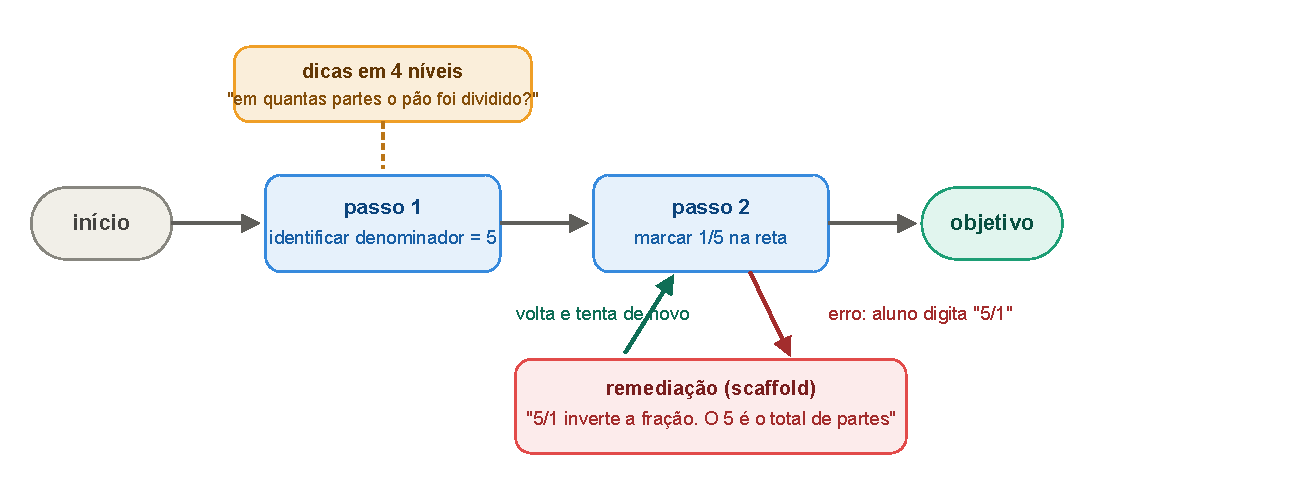
\includegraphics[width=\linewidth]{figures/figura-01.pdf}
  \caption{Anatomia de um grafo de comportamento. O caminho horizontal representa uma resolução correta; o desvio inferior associa uma misconception à remediação e ao retorno; o bloco superior representa uma cadeia progressiva de dicas. A figura é conceitual: os agentes avaliados propõem conteúdo, enquanto o GraphForge monta a topologia.}
  \label{fig:anatomia}
\end{figure}
\FloatBarrier

A EducaOFF automatiza parte dessa autoria por meio de três agentes baseados em modelos de linguagem: o 3a propõe um traço correto, o 3b propõe erros, diagnósticos e remediações, e o 3c propõe hesitações e dicas. Esses agentes não criam sozinhos a topologia final. Um extrator reduz e reorganiza suas saídas; depois, o GraphForge cria nós, arestas, scaffolds e manifestos. Avaliar somente o grafo montado mistura pelo menos quatro fontes de variação: conteúdo gerado, contrato de entrada, perdas no extrator e regras determinísticas do montador.

Por concisão, a expressão ``grafos gerados pelos agentes'' designa neste artigo os grafos produzidos pelo \textbf{fluxo assistido por agentes}: conteúdo proposto por 3a, 3b e 3c, transformado pelo extrator e montado pelo GraphForge. Ela não significa que o modelo de linguagem, isoladamente, produza a topologia final. Essa precisão é necessária para atribuir a qualidade --- ou a falha --- ao estágio em que ela efetivamente surge.

Neste trabalho, validar tecnicamente o processo de autoria de um grafo de comportamento significa reunir evidências separadas sobre: (a) o conteúdo do caminho correto; (b) a cobertura, o diagnóstico e a remediação de comportamentos errôneos; (c) a progressividade e a segurança dos scaffolds de dicas; (d) a preservação dessas informações até o artefato montado; e (e) a integridade estrutural e a reprodutibilidade da montagem. Cada dimensão é necessária para um grafo utilizável, mas nenhuma, isoladamente, estabelece validade pedagógica. Essa definição impede que topologia bem formada mas vazia, conteúdo plausível perdido no transporte ou montagem determinística de informações inadequadas sejam confundidos com um ``bom grafo''.

Versões anteriores deste trabalho mediram o subsistema integrado em uma bancada adaptada, mas não preservaram sem perdas as três saídas brutas. A Campanha 4 corrige essa limitação ao executar o código e as configurações da imagem implantada, congelar as saídas antes de abrir as referências CTAT e calcular métricas próprias para cada papel. A pergunta central é: \textbf{em que medida o fluxo legado de autoria assistida da EducaOFF produz componentes observáveis de um grafo de comportamento concordantes com a referência CTAT, preservados no transporte e estruturalmente reproduzíveis?} Ela é decomposta nas seguintes subperguntas:

\begin{enumerate}[label=\textbf{QP\arabic*.}]
  \item \textbf{Caminho correto:} em que medida o 3a produz uma sequência concreta concordante com o BRD?
  \item \textbf{Ramos buggy e remediação:} em que medida o 3b recupera valores errados da referência e emite informação remediativa utilizável?
  \item \textbf{Scaffold de dicas:} em que medida o 3c produz cadeias completas, distintas e sem revelação prematura da resposta?
  \item \textbf{Fidelidade de transporte:} que conteúdo e identidade de problema são preservados da saída bruta até a configuração e o artefato GraphForge?
  \item \textbf{Fidelidade e estrutura:} a execução corresponde ao código, às configurações e ao fluxo legado implantados, e a montagem é reprodutível?
  \item Um painel cego de LLMs acrescenta evidência auxiliar de qualidade textual às métricas determinísticas?
\end{enumerate}

A contribuição central não é um escore único de ``qualidade do grafo'', mas um perfil de evidências de validação por componente. O trabalho oferece uma decomposição auditável entre geração, concordância com referência, propriedades intrínsecas das dicas, transporte e montagem. Essa decomposição também define o limite da alegação: concordar com um BRD de autoria humana é evidência de alinhamento a uma referência, mas não prova que o BRD seja completo nem que comportamentos alternativos sejam inválidos. Avaliação humana independente e dados de estudantes continuam necessários para validade pedagógica.

\section{Fundamentação e escopo de validade}

\subsection{Grafo de comportamento, saída de agente e grafo final}

Um grafo de conhecimento organiza habilidades e pré-requisitos entre exercícios. Um grafo de comportamento, por sua vez, representa estados, ações, erros e intervenções em um exercício. O presente estudo trata apenas do segundo objeto. Mesmo assim, é necessário distinguir o conteúdo proposto pelos agentes da estrutura criada pelo montador. A Figura~\ref{fig:pipeline} explicita as fronteiras observadas.

\begin{figure}[tbp]
  \centering
  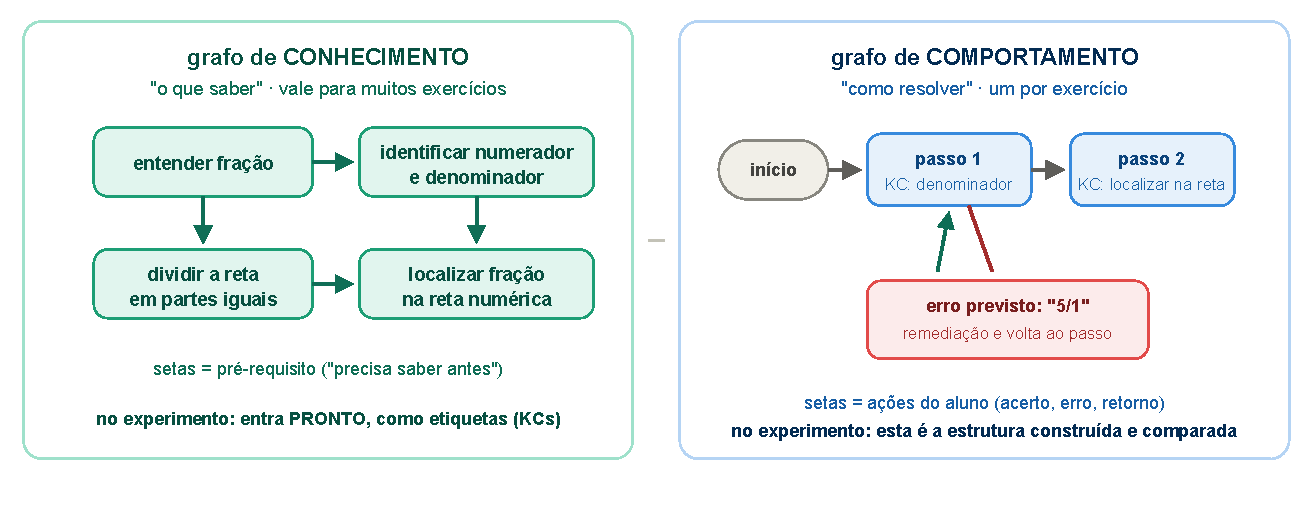
\includegraphics[width=\linewidth]{figures/figura-02.pdf}
  \caption{Diferença entre grafo de conhecimento (currículo e pré-requisitos compartilhados) e grafo de comportamento (estados e ações de um exercício). O estudo não avalia a criação de um grafo de conhecimento.}
  \label{fig:conhecimento-comportamento}
\end{figure}
\FloatBarrier

\begin{figure}[tbp]
\centering
\resizebox{\textwidth}{!}{%
\begin{tikzpicture}[
  node distance=6mm and 8mm,
  box/.style={draw=ruleblue,rounded corners=2pt,fill=softblue,align=center,minimum height=10mm,text width=26mm,font=\small},
  agent/.style={draw=ruleblue,rounded corners=2pt,fill=softgreen,align=center,minimum height=10mm,text width=25mm,font=\small},
  ref/.style={draw=red!55!black,dashed,rounded corners=2pt,fill=softred,align=center,minimum height=10mm,text width=28mm,font=\small},
  arrow/.style={-{Latex[length=2.2mm]},thick,draw=ruleblue},
  dasharrow/.style={-{Latex[length=2.2mm]},thick,dashed,draw=red!55!black}
]
\node[box] (state) {estado de autoria\\4 problemas-semente};
\node[agent,right=of state,yshift=13mm] (a) {Agente 3a\\traço correto};
\node[agent,right=of state] (b) {Agente 3b\\erros e remediação};
\node[agent,right=of state,yshift=-13mm] (c) {Agente 3c\\hesitações e dicas};
\node[box,right=12mm of b] (raw) {saídas brutas\\fechadas por hash};
\node[box,right=of raw] (extract) {extrator\\configuração};
\node[box,right=of extract] (forge) {GraphForge\\topologia e manifestos};
\node[ref,below=18mm of raw] (brd) {BRD CTAT\\referência de autoria};
\node[box,right=of brd] (metrics) {métricas por agente\\e por transporte};
\draw[arrow] (state) -- (a);
\draw[arrow] (state) -- (b);
\draw[arrow] (state) -- (c);
\draw[arrow] (a.east) -- (raw.west);
\draw[arrow] (b.east) -- (raw.west);
\draw[arrow] (c.east) -- (raw.west);
\draw[arrow] (raw) -- (extract);
\draw[arrow] (extract) -- (forge);
\draw[dasharrow] (brd) -- (metrics);
\draw[arrow] (raw.south) |- (metrics.west);
\draw[arrow] (forge.south) |- (metrics.east);
\node[font=\scriptsize,align=center,below=1mm of brd] {inacessível durante a autoria};
\end{tikzpicture}
}
\caption{Fluxo efetivamente avaliado. Os agentes produzem conteúdo candidato; o extrator e o GraphForge transformam esse conteúdo. O BRD entra somente depois do fechamento das saídas, na etapa de comparação. Agentes posteriores que adaptam o tutor final e a rota atual \emph{tool-first} estão fora do escopo.}
\label{fig:pipeline}
\end{figure}
\FloatBarrier

\subsection{Modelo de validação técnica em camadas}

A unidade conceitual de validação é o processo que forma o grafo e seus artefatos intermediários, não apenas o arquivo final. Como os agentes propõem componentes sem emitir a topologia CTAT completa, uma comparação monolítica entre ``grafo do agente'' e BRD atribuiria ao modelo decisões do extrator e do GraphForge. A Tabela~\ref{tab:validation-model} explicita a ligação entre anatomia do grafo, evidência observada e alcance da inferência. Não há limiar global de aprovação nem regra pós-hoc de ``válido/inválido''.

\begin{table}[tbp]
\centering
\caption{Modelo de validação técnica do grafo de comportamento.}
\label{tab:validation-model}
\small
\setlength{\tabcolsep}{3pt}
\begin{tabularx}{\textwidth}{@{}P{2.35cm}P{2.8cm}Y Y@{}}
\toprule
Camada & Componente observado & Evidência produzida & O que não demonstra \\
\midrule
Fidelidade de produção & código, configuração, entrada e política & identidade por digest e hashes do fluxo auditado & réplica externa byte a byte da imagem não publicada \\
Caminho correto & saída 3a e resposta final & instanciação concreta e concordância com ações corretas da referência & correção matemática abstrata de templates genéricos \\
Ramos buggy & saída 3b, diagnóstico e remediação & cobertura por valor do catálogo do BRD e presença de campos remediativos & validade de excedentes ou concordância por estado/SAI \\
Scaffold de dicas & saída 3c & completude, distinção, progressividade formal e vazamento literal & efeito das dicas sobre a aprendizagem \\
Transporte & configuração, grafo e manifesto de slots & retenção de conteúdo, campos e identidade de problema & qualidade pedagógica do conteúdo preservado \\
Montagem & topologia GraphForge & invariantes implementadas e identidade em reexecução & validade semântica ou pedagógica do grafo \\
\bottomrule
\end{tabularx}
\end{table}
\FloatBarrier

Para responder à questão prática de qualidade, o estudo usa uma síntese interpretativa pós-hoc com três estatutos: \textbf{evidência favorável no limite testado}, quando a propriedade foi observada sem defeito crítico conhecido; \textbf{fragilidade observada}, quando ausências ou falhas mensuradas comprometem o uso pretendido; e \textbf{não estimável}, quando a fonte externa necessária não existe. Como não foi congelado um limiar global de aprovação, esses estatutos não constituem teste de hipótese nem nota composta. A conclusão ``não pronto para uso autônomo'' é uma conclusão de risco de engenharia: basta que propriedades essenciais de executabilidade, segurança ou rastreabilidade estejam comprometidas; ela não afirma que todo conteúdo gerado seja pedagogicamente incorreto.

\subsection{O papel legítimo e limitado dos BRDs}

Os BRDs foram produzidos para tutores CTAT e constituem uma referência tecnicamente pertinente quando a pergunta é se o sistema reproduz os comportamentos registrados nesses tutores. Seu uso é particularmente informativo para ações concretas corretas e valores errados observáveis. Contudo, um único grafo não enumera necessariamente todas as soluções ou misconceptions pedagogicamente defensáveis. A discordância entre avaliadores qualificados pode refletir ambiguidade da tarefa, não apenas erro (Amidei; Piwek; Willis, 2018).

Por isso, este artigo usa os termos \textbf{concordância}, \textbf{recall da referência} e \textbf{cobertura}, nunca ``correção universal''. A identidade, a credencial do autor original e a licença específica dos BRDs não constam de modo suficiente no pacote recebido. O corpus é denominado ``referência CTAT''; a expressão ``padrão-ouro especialista'' não é usada. Uma demonstração de equivalência a especialistas exigiria múltiplos autores independentes, uma banda humano--humano e margem prospectiva de não inferioridade (Shavelson; Webb, 1991).

\subsection{Não inferioridade e banda humano--humano}

Quando não há um único grafo correto, igualdade exata com um autor não é um critério adequado de validade. A pergunta formal relevante seria se a divergência do sistema excede a divergência observada entre autores humanos independentes. Esse enquadramento requer uma margem de não inferioridade justificada antes da análise (Lakens, 2017; Lakens; Scheel; Isager, 2018) e uma estimativa da variabilidade entre autores. Pela Teoria da Generalizabilidade, um único grafo humano por exercício não permite separar a faceta exercício da faceta autor (Shavelson; Webb, 1991). Consequentemente, a não inferioridade permanece \textbf{não estimável} nas quatro campanhas. Os intervalos de concordância reportados não devem ser convertidos em um limiar informal de aprovação.

\subsection{Comparação assimétrica e territórios de divergência}

Métricas simétricas, como F1, penalizam todo item produzido que não apareça na referência. Isso mistura duas situações distintas: uma alucinação inválida e uma alternativa pedagogicamente plausível não registrada pelo autor. A comparação assimétrica de Tversky (1977) motiva separar três territórios: interseção, excedentes do sistema e omissões em relação à referência. As Campanhas 1--3 usaram cobertura por valor, inclusão de traços e F1 como medidas históricas; a Campanha 4 substitui o escore agregado por métricas específicas de cada agente e por retenção de campos. Em nenhum caso um excedente é automaticamente verdadeiro ou falso: sua validade exige outra fonte de evidência.

\subsection{Integridade estrutural como camada independente}

Propriedades topológicas podem ser testadas sem assumir que o conteúdo do BRD seja completo. O verificador do projeto procura violações duras --- ciclo fora de remediação, nó inalcançável, beco sem saída, scaffold ou aresta órfãos e ausência de início ou objetivo --- e sinais moles, como ramificação excessiva. Testes de propriedades sobre 10.000 configurações e mutation testing com 260 defeitos injetados exercitam as classes implementadas. Essa evidência demonstra consistência entre montador e verificador para a taxonomia coberta; não prova ausência de defeitos desconhecidos nem qualidade pedagógica. A Campanha 4 acrescenta uma verificação distinta: identidade byte a byte em reexecuções do mesmo GraphForge.

\subsection{LLMs como juízes auxiliares}

LLMs podem aplicar rubricas em escala, mas carregam vieses de preferência, família e estilo. Há evidência de que avaliadores reconhecem e favorecem produções da própria família (Panickssery; Bowman; Feng, 2024), e nem mesmo preferência humana agregada representa automaticamente todos os critérios de validade (Hosking; Blunsom; Bartolo, 2024). Neste estudo, os juízes pertencem a famílias diferentes da geradora, recebem códigos opacos e não veem o GraphForge. Ainda assim, suas notas são tratadas como evidência auxiliar. Mutações sintéticas medem sensibilidade a degradações óbvias; não substituem calibração com especialistas.

\section{Método}

\subsection{Programa de pesquisa e evolução do instrumento}

As quatro campanhas formam uma sequência de desenvolvimento, não quatro réplicas do mesmo experimento. As Campanhas 1 e 2 usaram um protocolo de dois envelopes derivados do BRD e avaliaram a bancada integrada; a Campanha 2 variou o modelo gerador. A Campanha 3 construiu a entrada sem ler o conteúdo do grafo de referência e introduziu uma bateria comportamental, mas continuou avaliando o subsistema depois de mapeamento e montagem. Essas três fases não retiveram de forma comparável todas as saídas de 3a, 3b e 3c. A Campanha 4 foi criada para fechar essa lacuna: usa o contrato multi-problema da rota legada, preserva saídas brutas e mede separadamente agente, extrator e GraphForge.

\begin{figure}[tbp]
\centering
\resizebox{\textwidth}{!}{%
\begin{tikzpicture}[
  node distance=9mm,
  phase/.style={draw=ruleblue,rounded corners=2pt,fill=softblue,align=center,minimum height=18mm,text width=34mm,font=\small},
  main/.style={draw=ruleblue,very thick,rounded corners=2pt,fill=softgreen,align=center,minimum height=18mm,text width=39mm,font=\small},
  arrow/.style={-{Latex[length=2.2mm]},thick,draw=ruleblue}
]
\node[phase] (c1) {Campanha 1\\piloto integrado\\cobertura e juiz único};
\node[phase,right=of c1] (c2) {Campanha 2\\robustez entre modelos\\mesmo protocolo v1};
\node[phase,right=of c2] (c3) {Campanha 3\\entrada independente\\conformidade integrada};
\node[main,right=of c3] (c4) {Campanha 4\\estudo principal\\agentes + transporte};
\draw[arrow] (c1) -- (c2);
\draw[arrow] (c2) -- (c3);
\draw[arrow] (c3) -- (c4);
\end{tikzpicture}%
}
\caption{Evolução do instrumento. As Campanhas 1--3 são fases históricas exploratórias; a Campanha 4 é a avaliação principal de componentes. A seta representa aprendizado metodológico, não comparabilidade direta dos estimandos.}
\label{fig:timeline}
\end{figure}
\FloatBarrier

\begingroup
\footnotesize
\setlength{\tabcolsep}{3pt}
\begin{longtable}{@{}P{1.15cm}P{2.65cm}P{3.0cm}P{3.25cm}P{1.65cm}P{2.55cm}@{}}
\caption{Comparabilidade e função das quatro campanhas.}\label{tab:campaigns}\\
\toprule
Fase & Objeto & Entrada & Desfecho central & Bruto preservado? & Identificação permitida \\
\midrule
\endfirsthead
\toprule
Fase & Objeto & Entrada & Desfecho central & Bruto preservado? & Identificação permitida \\
\midrule
\endhead
C1 & bancada integrada & envelope derivado do BRD & cobertura por valor; integridade; juiz histórico & não integralmente & piloto do instrumento \\
C2 & bancada integrada, quatro geradores & protocolo v1 & robustez exploratória da cobertura & não integralmente & contrastes entre braços da bancada \\
C3 & grafo integrado e executor analítico & interface e gabarito independentes do conteúdo do grafo & conformidade comportamental e ablações & insuficiente para atribuição & desempenho integrado sob protocolo v2 \\
C4 & agentes, extrator e GraphForge & contrato legado implantado com quatro problemas & métricas por agente e transporte & sim, antes da referência & diagnóstico direto por componente \\
\bottomrule
\end{longtable}
\endgroup

O corpus de 24 exercícios foi reutilizado. Logo, as campanhas não ampliam a amostra para 96 exercícios independentes. Entradas, runtime, unidade observacional, modelos auxiliares e estimandos também mudaram. Nenhuma estimativa é combinada entre campanhas, nenhum teste de tendência temporal é calculado e diferenças numéricas não são interpretadas como melhora ou piora do sistema. Os resultados históricos são apresentados porque documentam por que a separação da Campanha 4 se tornou necessária e permitem verificar se as novas observações oferecem mecanismos plausíveis para limitações antes vistas no agregado.

\subsection{Desenho, corpus e unidade de análise}

O corpus \path{frac-numberline-6.17} contém 24 exercícios sobre localização de frações na reta numérica. Enunciados e respostas esperadas foram materializados de uma chave independente derivada da interface, sem leitura dos BRDs. Quatro identificadores de KC foram construídos por regras de domínio: três comuns aos 24 exercícios e um adicional nos 12 casos de fração imprópria; cada exercício trazia três ou quatro KCs e quatro passos canônicos. Os exercícios foram agrupados em seis estados de quatro problemas, cardinalidade esperada pela rota implantada; em cada estado, as estratégias \path{polya}, \path{exemplo_trabalhado}, \path{problema_invertido} e \path{descoberta_guiada} aparecem uma vez.

Cada um dos seis estados foi planejado em três réplicas estocásticas, totalizando 18 unidades estado--réplica e 72 unidades exercício--réplica por agente. ``Réplica'' significa nova chamada com a mesma configuração; o runtime não expõe semente. A unidade inferencial registrada é o exercício, não a chamada nem cada passo. Primeiro se calcula a média das réplicas dentro do exercício; depois, a média macro dos 24 exercícios. Como quatro exercícios compartilham cada chamada, foi acrescentada após auditoria uma sensibilidade que reamostra os seis batches. Ela não substitui o intervalo registrado e, com apenas seis clusters, é descritiva e grosseira.

As métricas e o protocolo inicial dos juízes foram congelados antes da primeira chamada paga. Em seguida, três estados da réplica 1 foram executados como piloto; suas nove chamadas foram retidas no conjunto final. O plano das 45 chamadas geradoras restantes foi formalizado depois do piloto, usando apenas critérios operacionais previamente declarados de parse, custo e cobertura do gate, sem inspeção das métricas de qualidade. A Campanha 4 é, portanto, exploratória e auditável, mas não constitui um pré-registro integral concluído antes de qualquer coleta.

\subsection{Fidelidade à implantação e isolamento da referência}

A execução usou a imagem de contêiner \path{sha256:15b29e8063099d40fc62899da2795db6e97d3e252e486315428a0690bb9abf5b}. O \emph{filesystem diff} estava vazio. Os hashes dos agentes 3, do \path{pipeline-core}, do GraphForge e do catálogo de 33 misconceptions foram comparados com o manifesto antes de cada grupo. A imagem não contém rótulo VCS; o commit \path{7d3a676a94c3833bc95b1bde929d41bdbde94f1e} é um candidato fortemente corroborado, não identidade provada.

As chamadas ocorreram em cópia descartável da imagem, fora da VPS operacional. A credencial foi mantida em memória e não persistida nos artefatos. Cache, fallback e retries internos foram desabilitados. O preflight substituiu somente a chamada de rede por resposta simulada e congelou hashes das mensagens efetivas. O processo de autoria não podia abrir BRDs, envelopes históricos ou resultados anteriores; a referência CTAT era aplicada somente após persistência e fechamento das saídas brutas.

Uma auditoria posterior do depósito detectou que a atestação inicial da ontologia enumerava apenas três dos quatro identificadores de KC das fixtures. Segundo uma atestação operacional produzida pelo pesquisador, a consulta somente leitura do quarto identificador ao bridge implantado retornou HTTP 200 e vetor vazio nos três endpoints; durante a execução, o snapshot local respondeu 404 para esse identificador, resposta que o cliente de produção converte deterministicamente no mesmo vetor vazio. Assim, o enriquecimento efetivo permaneceu vazio nos dois ambientes, sem alteração dos grafos ou estimandos. Essa verificação é pós-hoc e não é externamente reproduzível com o depósito: as respostas HTTP brutas não foram preservadas. A omissão de cobertura no gate, a qualificação da evidência e os hashes do cliente constam da emenda \path{protocol/production-freeze-2026-07-15/AMENDMENT-C4-ONTOLOGY-KC4-POST-AUDIT-2026-07-15.md} e da atestação \path{protocol/production-freeze-2026-07-15/ontology-fixture-kc-attestation-v2.json}, SHA-256 \path{00dc41394488d56299a23e39fa14dccdd9dbfc369aab372b0651d80ef3f19394}.

\subsection{Agentes e configurações}

\begin{table}[H]
\centering
\caption{Papéis e configurações primárias da rota legada congelada.}
\label{tab:agents}
\small
\setlength{\tabcolsep}{3pt}
\begin{tabularx}{\textwidth}{@{}P{1.1cm}P{2.8cm}Y C{1.5cm}C{1.55cm}@{}}
\toprule
Agente & Papel & Saída principal & Temp. & Tokens máx. \\
\midrule
3a & aluno avançado & soluções com traço correto genérico, ações, resultados e KCs & 0,2 & 16.000 \\
3b & aluno em risco & tentativas, respostas erradas, diagnóstico, feedback e remediação & 0,7 & 24.000 \\
3c & aluno mediano & hesitações e cadeias de dicas em quatro níveis & 0,4 & 16.000 \\
\bottomrule
\end{tabularx}
\begin{minipage}{\textwidth}\footnotesize\emph{Nota.} Os três agentes usaram \path{google/gemini-3.5-flash} via OpenRouter no tier \emph{balanced}. As diferenças de temperatura pertencem à configuração implantada e não são fatores experimentais.
\end{minipage}
\end{table}

Os agentes 3a e 3b foram chamados em paralelo; o 3c seria chamado depois deles apenas se a política operacional não o pulasse. Como a condição operacional pulou o 3c em todos os estados completos, executou-se também um braço de \textbf{capacidade}: o mesmo agente e o mesmo prompt foram chamados diretamente, sem atribuir essa política à produção. As saídas de capacidade servem para avaliar o que o 3c consegue emitir; a política operacional serve para mostrar o que efetivamente chegaria ao restante do fluxo.

\subsection{Desfechos determinísticos}

A Tabela~\ref{tab:estimands} transforma o modelo conceitual em estimandos observáveis para cada componente do grafo. Nenhum escore composto foi criado, pois as camadas têm construtos e denominadores diferentes; portanto, seus valores não podem ser somados nem convertidos em uma nota global de validade.

\begingroup
\small
\setlength{\tabcolsep}{3pt}
\begin{longtable}{@{}P{2.6cm}P{3.0cm}P{4.6cm}P{4.55cm}@{}}
\caption{Componentes do grafo, desfechos e limites de interpretação.}\label{tab:estimands}\\
\toprule
Camada do grafo & Desfecho & Definição operacional & Interpretação permitida \\
\midrule
\endfirsthead
\toprule
Camada do grafo & Desfecho & Definição operacional & Interpretação permitida \\
\midrule
\endhead
Caminho correto (3a) & \Rthreea & $\LCS(E,G_c)/|E|$, com ações corretas concretas e ordenadas da referência ($E$) e resultados concretos gerados ($G_c$). Placeholders entre chaves recebem zero crédito. & Instanciação e concordância concreta; zero não implica, sozinho, erro matemático quando o contrato pede generalidade. \\
Caminho correto (3a) & resposta final & Igualdade exata, após canonização, entre \path{finalAnswer} e resposta esperada. & Diagnóstico secundário de instanciação. \\
Ramos buggy (3b) & \Rthreeb & Recall de valores errados concretos únicos presentes nas ações buggy comparáveis do BRD. & Cobertura da referência por valor; excedentes não são falsos automaticamente. \\
Localização buggy (3b) & proxy ordinal & Pareamento entre número ordinal do passo e valor. & Sensibilidade; não equivale a estado CTAT ou SAI. \\
Scaffold de dicas (3c) & \Cthreec por problema & Sucesso se há passo elegível e todas as cadeias são estritas: exatamente quatro níveis e tipos esperados, textos não vazios e distintos, sem resposta literal. & Qualidade operacional intrínseca; não mede aprendizagem. \\
Scaffold de dicas (3c) & completude e vazamento & Proporção de passos com níveis 1--4; proporção de dicas contendo literalmente a resposta final. & Diagnóstico de contrato e segurança pedagógica. \\
Transporte & retenção por campo & Correspondência exata entre saída bruta, configuração, grafo genérico e manifesto de slots. & Preservação de informação, não validade pedagógica. \\
Topologia GraphForge & determinismo & Identidade byte a byte do resultado em duas execuções da mesma configuração. & Reprodutibilidade do montador para os casos observados. \\
\bottomrule
\end{longtable}
\endgroup

O parser CTAT preservou estados e triplas SAI (\emph{Selection--Action--Input}). A referência contém 96 ações corretas comparáveis e 192 ações buggy, das quais 110 passaram o filtro primário de conteúdo; ações mecânicas e sentinelas exatas foram excluídas conforme regra congelada. O 3b não emite a combinação estado+SAI, de modo que o recall direto por estado planejado originalmente é \textbf{não estimável}. Substituí-lo silenciosamente pelo número do passo produziria uma alegação mais forte que os dados.

Para o 3c, passo elegível é aquele com \path{hesitation=true} ou dicas emitidas. Uma cadeia estrita exige níveis 1--4, tipos \path{conceptual}, \path{procedural}, \path{specific} e \path{bottom_out}, quatro textos distintos e ausência da resposta literal. A taxa de vazamento usa cada mensagem de dica como unidade descritiva; o sucesso estrito por problema usa exercício--réplica e entra como zero na ausência de estado.

\subsection{Falhas, análise \ITT{} e incerteza}

O plano determinou tentativa única, sem reparo, retry, fallback ou imputação para os geradores. Falha de chamada, parse ou estado atômico entra como zero/ausência no estimando \ITT. A análise restrita a estados completos é secundária. Intervalos de confiança percentis de 95\% foram obtidos por 20.000 reamostragens com reposição dos 24 exercícios, usando sementes fixas diferentes por métrica (Efron; Tibshirani, 1993). Esses intervalos quantificam estabilidade entre exercícios do corpus, mas não modelam a chamada compartilhada. A sensibilidade pós-hoc por batch preserva esse agrupamento; nenhum dos dois procedimentos corrige viés de seleção do domínio nem transforma o estudo em confirmatório.

\subsection{Painel auxiliar de qualidade textual}

Cada uma das 204 saídas principais observadas (68 por agente) foi apresentada separadamente a três famílias de juiz: \path{z-ai/glm-5.2}, \path{qwen/qwen3.7-plus} e \path{deepseek/deepseek-v4-pro}. O modelo gerador pertence à família Google. Os juízes receberam enunciado, resposta, KCs, passos independentes e a saída bruta do respectivo agente, mas não receberam identidade do agente, réplica, modelo, lote ou artefato GraphForge. A ordem foi derivada deterministicamente de hash próprio por modelo.

Cada papel tinha cinco dimensões em escala ordinal 0--4. Para o 3a, os placeholders eram declarados intencionais e avaliados por coerência e transferibilidade; para o 3b, erros plausíveis não eram penalizados apenas por não aparecerem no BRD; para o 3c, a resposta esperada era mostrada para permitir detecção de revelação prematura. A agregação por dimensão é a mediana quando pelo menos dois juízes são válidos. Ausências não foram imputadas.

Como controle de sensibilidade, seis exercícios predeterminados receberam uma mutação por papel: contradição e remoção de passo no 3a; resposta errada igual ao gabarito e remoção de diagnóstico/remediação no 3b; e quatro dicas idênticas que entregam a resposta no 3c. Isso produziu 18 unidades mutadas e 54 julgamentos adicionais. Uma dimensão foi considerada sensível se a nota mutada caiu em pelo menos 80\% dos pares válidos. Foram calculados alfa ordinal de Krippendorff, kappa quadrático pareado, distribuição de escores e taxa de divergência maior que um ponto (Krippendorff, 2018). Com marginais quase constantes, estatísticas corrigidas pelo acaso são instáveis; por isso, distribuição e calibração têm prioridade interpretativa.

O protocolo do painel foi congelado antes dos resultados dos geradores, mas a composição de modelos foi alterada depois por custo. Três lançamentos técnicos parciais foram excluídos integralmente: v1 por keywords de JSON Schema não portáveis; v2 por limite de compilação de gramáticas remotas; e v4 após retirada de GPT-5.4. A execução final v5 começou do zero. Rubricas, unidades, mutações e análises permaneceram inalteradas. Trata-se, portanto, de evidência auxiliar pós-registro, não teste confirmatório.

\subsection{Rastreabilidade e testes}

Estados, prompts, respostas, usage, custos, erros, configurações intermediárias, grafos e manifestos foram preservados. Cada lançamento possui journal append-only e hashes SHA-256. A análise final foi executada depois do fechamento das saídas. Uma errata v2.1 corrigiu somente quatro taxas descritivas de campos do 3a; contagens, saídas, estimandos diretos e métricas de outras funções não mudaram. O código e os testes da versão v2 foram recuperados com os hashes exatos registrados no congelamento, respectivamente \path{4f8ae7d374bb08fe9ac59cedc622fde92f40379f635b47a05fc69d9044dfd6fa} e \path{eb9be4ff5f651b858e6b6d0038796bf930e67bab849132ad4af139803340b335}. Contudo, o JSON piloto v2 original, cujo hash começava por \path{35dee4}, foi sobrescrito e não pôde ser recuperado byte a byte; seus valores científicos permanecem recomputáveis, mas o timestamp original não. Uma errata analítica v5.1 preservou o painel original e marcou alfa/kappa como não estimáveis quando havia uma única categoria observada. Testes automatizados cobrem fixtures, contrato, identidade de produção, filtros CTAT, denominadores, transporte, segurança financeira e estatística.

\section{Resultados da validação técnica em camadas}

\subsection{Execução e falha preservada}

De 18 estados planejados, 17 foram concluídos (94,4\%). Na réplica 3 do batch 03, o provedor retornou as respostas de 3a e 3b, mas o JSON de 3b era malformado. O 3a foi aceito pelo parser antes da falha atômica; o 3c não foi chamado. O estado, que continha quatro exercícios, não foi repetido nem reparado. O 3a, portanto, retornou 72/72 soluções brutas identificáveis, mas somente 68/72 foram integradas e pontuadas sob a política atômica. Para 3b e 3c, 68/72 ficaram integráveis. As 72 unidades permanecem no denominador \ITT. Logo, o \ITT{} estima efetividade do pipeline atômico; o zero imposto ao 3a no estado falho não mede sua capacidade isolada.

\begin{table}[H]
\centering
\caption{Execução dos geradores na Campanha 4.}
\label{tab:execution}
\footnotesize
\setlength{\tabcolsep}{3pt}
\begin{tabularx}{\textwidth}{@{}P{1.8cm}R{1.15cm}R{1.45cm}R{1.45cm}R{1.55cm}R{1.55cm}Y@{}}
\toprule
Componente & N & Tokens entrada & Tokens saída & Custo (US\$) & Latência mediana & Estado \\
\midrule
Agente 3a & 18 & 42.540 & 36.254 & 0,3901 & 11,47 s & 18 respostas retornadas; 17 estados integrados \\
Agente 3b & 18 & 53.268 & 87.248 & 0,8651 & 30,22 s & uma resposta malformada \\
Agente 3c & 17 & 49.607 & 69.372 & 0,6988 & 23,46 s & não chamado no estado falho \\
\midrule
Total & 53 & 145.415 & 192.874 & 1,9540 & 23,22 s & 52 respostas aceitas pelo parser; 51 integradas \\
\bottomrule
\end{tabularx}
\begin{minipage}{\textwidth}\footnotesize\emph{Nota.} O percentil 95 da latência foi 34,0 s. Não houve retry nem fallback. Uma resposta 3a parseável ficou fora da análise integrada porque o estado falhou atomicamente.
\end{minipage}
\end{table}

\subsection{Validade de conteúdo por componente autorado}

\begingroup
\small
\setlength{\tabcolsep}{3pt}
\begin{longtable}{@{}P{1.2cm}P{4.7cm}C{1.75cm}C{2.1cm}P{3.9cm}@{}}
\caption{Métricas diretas, sem escore composto.}\label{tab:direct}\\
\toprule
Agente & Métrica & Estimativa & IC95\% bootstrap & Denominador/estatuto \\
\midrule
\endfirsthead
\toprule
Agente & Métrica & Estimativa & IC95\% bootstrap & Denominador/estatuto \\
\midrule
\endhead
3a & Recall concreto ordenado \ITT{} & 0,000 & [0,000; 0,000] & 24 exercícios, 72 unidades \ITT{} \\
3a & Igualdade exata da resposta final \ITT{} & 0,111 & [0,028; 0,222] & 24 exercícios, 72 unidades \ITT{} \\
3a & Resultados genéricos entre saídas integradas & 1,000 & [1,000; 1,000] & 68 saídas pontuáveis \\
3b & Recall de valores errados únicos \ITT{} & 0,176 & [0,113; 0,242] & 24 exercícios, 72 unidades \ITT{} \\
3b & Recall de valores, estados completos & 0,190 & [0,124; 0,260] & 68 saídas observadas \\
3b & Proxy ordinal passo--valor \ITT{} & 0,060 & [0,023; 0,105] & sensibilidade; não é estado CTAT \\
3c & Sucesso estrito por problema \ITT{} & 0,278 & [0,167; 0,403] & braço de capacidade; 72 unidades \ITT{} \\
3c & Sucesso estrito, estados completos & 0,299 & [0,188; 0,424] & braço de capacidade; 68 saídas \\
3c & Completude 1--4 condicional & 1,000 & [1,000; 1,000] & 82 passos elegíveis \\
3c & Validade estrita condicional & 0,382 & [0,257; 0,507] & média macro; cadeias emitidas \\
3c & Vazamento literal da resposta & 0,226 & [0,172; 0,285] & média macro; dicas emitidas \\
\bottomrule
\end{longtable}
\endgroup

Na sensibilidade pós-hoc que reamostrou os seis batches de chamada, a estimativa pontual foi preservada, mas o IC do acerto final do 3a ampliou-se para [0,000; 0,333]; os intervalos do recall do 3b e do sucesso estrito do 3c foram, respectivamente, [0,117; 0,244] e [0,153; 0,444]. Os valores registrados por exercício continuam sendo os resultados principais da Tabela~\ref{tab:direct}; a sensibilidade mostra que a precisão do 3a foi superestimada quando a dependência intra-chamada foi ignorada.

\paragraph{Agente 3a.} Todos os resultados intermediários emitidos continham placeholders como \path{\{A\}}, \path{\{B\}} e \path{\{C\}}, conforme exigência explícita do prompt. Consequentemente, a LCS concreta foi zero em todas as unidades. Esse resultado diagnostica incompatibilidade entre um contrato de traço genérico e uma referência de ações concretas; não permite afirmar que as relações abstratas eram matematicamente erradas. A baixa correspondência da resposta final (11,1\%) confirma, contudo, que a saída não está pronta para execução concreta sem uma etapa de instanciação validada.

\paragraph{Agente 3b.} O agente emitiu 136 erros concretos observados, e nenhum tinha \path{wrongAnswer} igual à resposta correta. O recall macro dos valores registrados no BRD foi 17,6\% sob \ITT{} e 19,0\% entre estados completos. A referência pode omitir erros plausíveis; por isso, o complemento não é ``taxa de erro'' do agente. O resultado demonstra apenas baixa recuperação do catálogo específico. A concordância por estado/SAI permanece não estimável porque o contrato não emite estado e tripla SAI CTAT; isso é distinto da perda posterior de \path{problemId} no extrator.

\paragraph{Agente 3c.} Os 82 passos elegíveis continham 328 dicas e todos apresentavam quatro níveis. Apenas 32 cadeias satisfizeram simultaneamente os critérios estritos; 75 mensagens continham a resposta final literal. As taxas agrupadas por item (39,0\% de cadeias estritas e 22,9\% de vazamento) são próximas, mas não idênticas, às médias macro da Tabela~\ref{tab:direct}. A completude formal dos quatro níveis, portanto, não garante progressividade, distinção ou ausência de entrega da resposta.

\subsection{Fidelidade de transporte e montagem GraphForge}

\begingroup
\small
\setlength{\tabcolsep}{3pt}
\begin{longtable}{@{}P{1.2cm}R{1.25cm}R{1.35cm}R{1.55cm}R{1.65cm}P{6.75cm}@{}}
\caption{Retenção ponderada por item da saída bruta ao artefato de destino.}\label{tab:transport}\\
\toprule
Agente & Bruto & Config. & Destino & Retenção bruto--config. & Perdas e campos críticos \\
\midrule
\endfirsthead
\toprule
Agente & Bruto & Config. & Destino & Retenção bruto--config. & Perdas e campos críticos \\
\midrule
\endhead
3a & 272 & 60 & 60 nós & 22,1\% & 212 itens truncados; ação e KC chegam aos nós, mas resultado e índice original não; \path{problemId} não chega à configuração. \\
3b & 136 & 117 & 117 erros & 86,0\% & 19 itens perdidos por ausência de ID, deduplicação ou truncamento; pergunta diagnóstica, localização e \path{problemId} não chegam à configuração; registros restantes chegam integralmente ao grafo. \\
3c capacidade & 328 & 272 & 272 dicas no manifesto & 82,9\% & nível, tipo e \path{problemId} são perdidos; textos ficam no \path{slotManifest.existingHints}; nenhum texto aparece nos nós do grafo genérico. \\
3c operacional & 328\textsuperscript{a} & 0 & 0 & 0,0\% & a política implantada pulou o 3c em todos os 17 estados completos; nenhuma dica seguiria no fluxo operacional. \\
\bottomrule
\multicolumn{6}{P{14.6cm}}{\footnotesize\textsuperscript{a} Os 328 itens existem no braço forçado de capacidade. A linha operacional aplica a decisão real de skip ao mesmo conjunto de estados; ela não significa que a produção ordinária tenha chamado o 3c.}\\
\end{longtable}
\endgroup

O corte do 3a ocorre antes do GraphForge, no extrator que concatena soluções e retém um prefixo global. Entre configuração e grafo, ações e KCs são preservados, mas resultados concretos deixam de existir como campo de nó. Para o 3b, a maior parte do registro reduzido chega ao grafo, porém campos pedagogicamente relevantes já foram descartados. Para o 3c, a topologia genérica não transporta dicas; somente o manifesto de slots conserva textos, sem nível nem tipo. Em todos os agentes, a perda de \path{problemId} impede rastrear com segurança a origem depois da fusão multi-problema.

O GraphForge produziu resultados idênticos em 34/34 pares de reexecução, cobrindo as políticas operacional e de capacidade nos 17 estados completos. Isso sustenta determinismo observado do montador; não recupera dados removidos pelo extrator nem prova correção pedagógica da topologia.

\subsection{Juízo sobre a qualidade dos grafos produzidos}

As métricas por agente respondem a componentes diferentes do mesmo objeto final. Para o caminho correto, o 3a não produziu instanciação concreta concordante nas ações intermediárias e acertou a resposta final em 11,1\% das unidades \ITT{}, embora isso não permita condenar a correção abstrata de seus templates. Para os ramos buggy, o 3b recuperou 17,6\% dos valores de erro da referência e não forneceu identidade estado/SAI suficiente para localizar esses ramos no grafo CTAT. Para o scaffold, o 3c sempre formou quatro níveis quando emitiu uma cadeia, mas a média macro por exercício da validade estrita entre cadeias observadas foi 38,2\% e a média macro da taxa de vazamento literal entre dicas emitidas foi 22,6\%; sua contribuição ao fluxo operacional foi nula nos 17 estados completos porque a política o pulou.

Esses conteúdos ainda sofreram transformação antes do artefato final: a retenção bruto--configuração foi 22,1\% no 3a, 86,0\% no 3b e 82,9\% no braço de capacidade do 3c, com perda universal de \path{problemId}. O GraphForge repetiu a montagem de forma idêntica em 34/34 pares, mas montou somente o que sobreviveu ao extrator. Portanto, a evidência sustenta uma validação técnica \textbf{parcial e localizada}: identifica quais componentes do grafo estão presentes, ausentes ou não rastreáveis, sem fornecer base para aprovar o grafo para publicação autônoma. Inversamente, a referência de autor único também não permite declarar que todo comportamento excedente seja pedagogicamente inválido.

O estudo não pré-especificou um escore composto nem um limiar global de aprovação; portanto, não se estima uma proporção de ``grafos corretos''. Ainda assim, as métricas permitem responder qualitativamente à pergunta sobre sua qualidade. Um grafo utilizável requer simultaneamente caminho correto executável, erros localizados, intervenções adequadas, preservação da identidade do problema e montagem íntegra. Na versão auditada, somente a regularidade das saídas e a reprodutibilidade da montagem receberam evidência favorável, e mesmo a primeira não foi livre de falhas. As demais dimensões necessárias ao comportamento do tutor apresentaram fragilidades ou permaneceram não estimáveis. A Tabela~\ref{tab:quality-verdict} torna explícita essa síntese interpretativa; ela reorganiza resultados já apresentados e não introduz novo estimando.

\begingroup
\small
\setlength{\tabcolsep}{3pt}
\begin{longtable}{@{}P{2.65cm}P{4.55cm}P{3.15cm}P{4.15cm}@{}}
\caption{Perfil pós-hoc de qualidade dos grafos produzidos pelo fluxo auditado.}\label{tab:quality-verdict}\\
\toprule
Dimensão necessária & Evidência observada & Estatuto & Consequência para o grafo \\
\midrule
\endfirsthead
\toprule
Dimensão necessária & Evidência observada & Estatuto & Consequência para o grafo \\
\midrule
\endhead
Regularidade da geração & 17/18 estados concluídos; 52 respostas aceitas pelo parser e 51 saídas integradas; uma resposta 3b malformada & favorável no limite testado, com falha observada & o fluxo normalmente produz artefatos processáveis, mas não é livre de falhas de geração ou integração \\
Caminho correto executável & recall concreto intermediário 0; correspondência exata da resposta final 0,111; resultados intermediários genéricos em 1,000 das saídas integradas & fragilidade observada & o grafo não recebe do 3a um traço concreto suficiente para execução direta; isso não prova erro abstrato dos templates \\
Ramos buggy localizados & recall por valor 0,176; identidade estado/SAI não estimável; nenhum dos 136 erros emitidos coincidiu com a resposta correta & fragilidade observada & há candidatos de erro potencialmente úteis, mas cobertura e localização são insuficientes para uso automático confiável \\
Scaffold seguro e utilizável & sucesso estrito por problema 0,278; médias macro por exercício de 0,382 para validade estrita condicional e 0,226 para taxa de vazamento literal; 3c pulado nos 17 estados completos & fragilidade observada & completude formal das cadeias não garante progressão segura, e o grafo operacional observado não recebeu as dicas \\
Rastreabilidade e transporte & retenção 22,1\%/86,0\%/82,9\% para 3a/3b/3c-capacidade; \path{problemId} perdido nos três fluxos; nível, tipo e localização também descartados & fragilidade crítica observada & conteúdo não pode ser atribuído com segurança ao exercício ou ao ponto comportamental de origem depois da fusão \\
Montagem reprodutível & 34/34 pares de reexecução GraphForge idênticos & favorável no limite testado & a mesma entrada sobrevivente produz o mesmo artefato; determinismo não recupera perdas nem valida semântica \\
Plausibilidade textual & painel com forte efeito teto, dez dimensões degeneradas e sensibilidade em seis de oito dimensões mutadas & evidência auxiliar inconclusiva & notas altas não autorizam aprovação do conteúdo ou do grafo \\
Adequação pedagógica & ausência de novos especialistas independentes e de estudo com estudantes & não estimável & não se pode afirmar validade pedagógica, eficácia educacional ou equivalência a especialistas \\
\midrule
Juízo global & forma geralmente processável e montagem estável, mas conteúdo comportamental incompleto, segurança inconsistente e rastreabilidade insuficiente & \textbf{não pronto para uso autônomo} & papel defensável: rascunho assistivo submetido a gates automáticos e revisão humana antes da implantação \\
\bottomrule
\end{longtable}
\endgroup

Esse juízo é deliberadamente assimétrico. Ele não afirma que todos os grafos ou todos os conteúdos excedentes sejam pedagogicamente errados. Afirma que as propriedades essenciais observadas não foram satisfeitas em conjunto e que, por isso, os dados não sustentam tratar o artefato final como um tutor autorado autonomamente e pronto para publicação.

\subsection{Painel auxiliar de juízes}

O painel final executou 666 unidades primárias e 102 reparos, totalizando 768 chamadas. Houve 601 julgamentos válidos e 65 ausentes. Qwen e DeepSeek completaram 222/222 unidades cada um, sem reparo. GLM completou 157/222; 102 de suas respostas iniciais exigiram reparo e 65 permaneceram inválidas. Entre as ausências finais do GLM, 59 decorreram de \path{confidence} fora do intervalo local 0--1 e seis de JSON malformado. Todas as 204 unidades principais conservaram pelo menos dois juízes válidos.

\begin{table}[H]
\centering
\caption{Cobertura e custo do painel auxiliar v5.}
\label{tab:judges}
\small
\setlength{\tabcolsep}{3pt}
\begin{tabularx}{\textwidth}{@{}Y R{1.35cm}R{1.45cm}R{1.35cm}R{1.35cm}R{1.8cm}@{}}
\toprule
Juiz & Unid. & Válidas & Reparos & Ausentes & Custo (US\$) \\
\midrule
GLM-5.2 & 222 & 157 & 102 & 65 & 0,7964 \\
Qwen 3.7 Plus & 222 & 222 & 0 & 0 & 0,1901 \\
DeepSeek V4 Pro & 222 & 222 & 0 & 0 & 0,2567 \\
\midrule
Total & 666 & 601 & 102 & 65 & 1,2432 \\
\bottomrule
\end{tabularx}
\begin{minipage}{\textwidth}\footnotesize\emph{Nota.} O custo contábil público canônico usa preços-teto congelados. Uma variação de uso da chave de US\$ 0,9955 consta apenas de registro privado de conta, omitido do depósito público, e não é usada como estimativa de custo do painel. O painel permaneceu abaixo da trava de execução de US\$ 3. Não houve fallback.
\end{minipage}
\end{table}

As medianas agregadas foram 4 em todas as 15 dimensões. Entre avaliações válidas, o escore 4 correspondeu a 99,79\% das notas do 3a, 99,67\% das notas do 3b e 99,54\% das notas do 3c (2.746/2.755 notas no total). Dez das 15 dimensões usaram somente a categoria 4. Nelas, $D_o=D_e=0$: não há variação suficiente para estimar confiabilidade corrigida pelo acaso. Trinta e três dos 45 kappas pareados são igualmente degenerados. Nas cinco dimensões restantes, o alfa ordinal variou de $-0{,}0055$ a 0,3294. A concordância quadrática bruta ponderada variou de 0,9856 a 1,000, e apenas duas dimensões tiveram uma unidade com divergência maior que um ponto. A combinação de teto, marginais degeneradas e perdas seletivas do GLM torna enganosa qualquer leitura de ``confiabilidade perfeita''; unanimidade bruta sob uma única categoria não demonstra poder discriminativo.

\begingroup
\small
\setlength{\tabcolsep}{3pt}
\begin{longtable}{@{}P{2.8cm}P{4.0cm}C{1.1cm}C{1.35cm}C{1.55cm}P{2.2cm}@{}}
\caption{Calibração por mutações sintéticas; $\Delta=$ nota mutada menos nota original.}\label{tab:mutations}\\
\toprule
Papel & Dimensão alvo & Pares & $\overline{\Delta}$ & Queda & Gate 80\% \\
\midrule
\endfirsthead
\toprule
Papel & Dimensão alvo & Pares & $\overline{\Delta}$ & Queda & Gate 80\% \\
\midrule
\endhead
Traço correto & correção/coerência & 14 & $-4,000$ & 14/14 & passou \\
Traço correto & cobertura/ordem & 14 & $-3,000$ & 14/14 & passou \\
Erros/remediação & plausibilidade do erro & 15 & 0,000 & 0/15 & \textbf{falhou} \\
Erros/remediação & diagnóstico causal & 15 & 0,000 & 0/15 & \textbf{falhou} \\
Erros/remediação & remediação acionável & 15 & $-3,200$ & 15/15 & passou \\
Dicas & progressão de scaffold & 15 & $-3,600$ & 15/15 & passou \\
Dicas & distinção & 15 & $-3,533$ & 15/15 & passou \\
Dicas & não vazamento & 15 & $-3,867$ & 15/15 & passou \\
\bottomrule
\end{longtable}
\endgroup

Os juízes detectaram contradições, remoção de passo, remediação vazia e dicas repetitivas com entrega da resposta. Porém, quando a resposta errada foi substituída pela resposta correta e \path{diagnosticQuestion}/\path{howToFix} foram removidos, eles não reduziram plausibilidade nem diagnóstico causal. A mutação ainda preservava descrição e localização do erro; portanto, esse controle testa degradação parcial, não ausência total de evidência causal. O painel passou em seis de oito dimensões mutadas; sete das 15 dimensões da rubrica não foram alvo de mutação. Em conjunto, o resultado apoia apenas uma conclusão estreita: os textos principais pareceram bem formados e coerentes para os modelos, mas as notas absolutas têm baixa capacidade discriminativa e não podem validar pedagogicamente os agentes.

\subsection{Custos e lançamentos excluídos}

O custo contábil do experimento analítico foi US\$ 1,9540 para geração e US\$ 1,2432 para o painel final. Três lançamentos técnicos de juízes foram preservados e excluídos universalmente: v1 (58 tentativas concluídas, dois escores válidos, US\$ 0,00245 contabilizado), v2 (329 concluídas, 240 válidas, US\$ 1,80965) e v4 (124 concluídas, todas válidas, US\$ 0,40896). O overhead conhecido excluído soma US\$ 2,22106; chamadas diagnósticas e tentativas em voo impedem tratá-lo como custo financeiro total exato. Nenhum escore desses lançamentos foi usado para selecionar unidades, rubricas ou conclusões. A trava lógica de US\$ 3 do painel era verificada após a conclusão de cada tarefa; com concorrência nove, chamadas já em voo poderiam produzir pequeno \emph{overshoot}. Isso não ocorreu: o custo contábil final foi US\$ 1,2432.

\section{Campanhas 1--3: desenvolvimento e evidência histórica}

\subsection{Estatuto e função no manuscrito consolidado}

As Campanhas 1--3 são mantidas porque documentam o desenvolvimento do instrumento e resultados integrados que motivaram a Campanha 4. Elas não são usadas para confirmar as estimativas atuais, escolher métricas retrospectivamente ou ampliar o tamanho amostral. Todas empregaram os mesmos 24 exercícios, com três réplicas por condição, mas variaram fonte de entrada, modelos, preparação da configuração e objeto medido. Na bancada histórica, os agentes alimentavam um adaptador experimental antes do GraphForge; portanto, suas métricas caracterizam a cadeia integrada sob aquele adaptador, não a capacidade isolada de 3a, 3b ou 3c.

O protocolo v1, usado nas Campanhas 1 e 2, separava o BRD em dois envelopes: um envelope de entrada com interface, resposta correta e KCs, e um envelope de referência aberto somente para comparação. A lista de campos proibidos e testes de vazamento impediam acesso lexical às misconceptions, dicas e arestas. Todavia, ambos os envelopes eram derivados do mesmo arquivo; havia blindagem parcial, não independência de fonte. Na Campanha 3, a entrada passou a ser construída a partir da interface e do gabarito de produção em massa, sem ler o conteúdo comportamental do BRD. Essa mudança removeu a dependência direta, mas alterou simultaneamente idioma, disponibilidade de KCs e representação da tarefa.

\subsection{Campanha 1: piloto do instrumento integrado}

A Campanha 1 verificou integridade estrutural, cobertura direcional do catálogo de valores e funcionamento de um juiz cego histórico. A média de completude conceitual foi 0,376 (IC95\% 0,309--0,442); a completude de passos foi 0,510 (0,497--0,525). O kappa médio da classificação sobre a união dos catálogos foi 0,007 ($-0,069$ a 0,089), resultado essencialmente nulo. A bateria não possuía verdadeiros negativos por construção, o que limita, mas não transforma o kappa baixo em concordância positiva.

\begingroup
\small
\setlength{\tabcolsep}{3pt}
\begin{longtable}{@{}P{6.6cm}C{3.0cm}P{4.6cm}@{}}
\caption{Síntese auditada da Campanha 1; 24 exercícios com três réplicas agregadas por exercício.}\label{tab:c1}\\
\toprule
Métrica & Estimativa [IC95\%] & Limite interpretativo \\
\midrule
\endfirsthead
\toprule
Métrica & Estimativa [IC95\%] & Limite interpretativo \\
\midrule
\endhead
Completude conceitual por valor & 0,376 [0,309; 0,442] & cobertura do catálogo de um autor, não correção universal \\
Completude bruta, incluindo registros mecânicos & 0,234 [0,195; 0,273] & sensível a sentinelas e ações de interface \\
Completude de passos & 0,510 [0,497; 0,525] & granularidade de passos difere entre artefatos \\
Concordância bruta de classificação & 0,396 [0,345; 0,449] & união de catálogos sem verdadeiros negativos \\
Kappa médio de Cohen & 0,007 [$-0,069$; 0,089] & não excede o acaso de modo demonstrável \\
Excedentes julgados plausíveis pelo GLM-4.5 & 0,83 [0,74; 0,91] & juiz único, sem calibração humana \\
\bottomrule
\end{longtable}
\endgroup

O juiz GLM-4.5 classificou 55 de 66 excedentes decididos como plausíveis, com dois empates excluídos; aprovou 82/83 itens da referência e rejeitou os 48 controles formados por resposta correta e valor absurdo. A taxa de 83\% significa apenas ``plausível segundo esse juiz e essa rubrica''. Em campanha posterior, outro juiz alterou substancialmente níveis absolutos de calibração e de centralidade das omissões. Por isso, a Campanha 1 não fornece validação pedagógica dos excedentes.

Um caso ilustra o significado de cobertura. Em \path{04soccerSeason}, cuja resposta é $3/4$, a referência registrava $2/4$, $3$ e $4$; o sistema produziu $2/4$, $3$ e $4/4$. Assim, cobriu dois de três valores conceituais, omitiu o denominador isolado e acrescentou uma confusão entre total de partes e fração. A comparação identifica interseção e divergências, mas não decide sozinha se $4/4$ deve integrar um tutor. O padrão do denominador isolado reapareceu em vários exercícios e motivou as análises por tipo de erro.

\subsection{Campanha 2: repetibilidade interna e variação do gerador}

A Campanha 2 repetiu o baseline e variou apenas o modelo usado nos três agentes da bancada. A nova execução do Gemini obteve completude conceitual de 0,368 (0,300--0,442), próxima da Campanha 1, 0,376 (0,309--0,442). Isso é repetibilidade interna no mesmo corpus, não replicação independente. Os braços históricos foram Gemini 3.5 Flash, GLM-5.2, DeepSeek V4 Pro e Claude Sonnet 5. A presença do Claude nesta seção é um fato da Campanha 2 e não significa que ele tenha participado da Campanha 4 ou do painel final v5.

\begingroup
\footnotesize
\setlength{\tabcolsep}{3pt}
\begin{longtable}{@{}P{3.35cm}C{2.35cm}C{2.35cm}C{2.35cm}C{2.35cm}@{}}
\caption{Resultados históricos por modelo gerador na Campanha 2.}\label{tab:c2-models}\\
\toprule
Métrica & Gemini & GLM-5.2 & DeepSeek V4 Pro & Claude Sonnet 5 \\
\midrule
\endfirsthead
\toprule
Métrica & Gemini & GLM-5.2 & DeepSeek V4 Pro & Claude Sonnet 5 \\
\midrule
\endhead
Completude conceitual & 0,368 [0,300; 0,442] & 0,415 [0,323; 0,504] & 0,371 [0,292; 0,454] & 0,416 [0,339; 0,488] \\
Completude de passos & 0,508 [0,493; 0,523] & 0,501 [0,479; 0,521] & 0,477 [0,458; 0,496] & 0,500 [0,487; 0,516] \\
Kappa médio & 0,051 & $-0,027$ & $-0,074$ & $-0,033$ \\
Excedentes plausíveis segundo Mistral & 0,74 & 0,78 & 0,73 & 0,73 \\
\bottomrule
\end{longtable}
\endgroup

Nenhuma diferença da completude conceitual primária foi detectada contra o baseline após Holm (p ajustado 0,988 nas três comparações). Isso não demonstra equivalência: os intervalos das diferenças ainda admitem efeitos relevantes. Entre métricas secundárias, somente a menor completude de passos do DeepSeek sobreviveu ao ajuste ($\Delta=-0,031$, p-Holm=0,035). Os níveis absolutos do juiz Mistral não são comparáveis aos do GLM-4.5 usado na Campanha 1. A principal conclusão é negativa e útil: trocar o modelo não removeu o teto de cobertura observado na bancada.

A anatomia da referência continha 83 instâncias conceituais únicas: 30 frações incorretas, 24 numeradores isolados, 24 denominadores isolados e cinco outros inteiros. Em uma execução do baseline, as coberturas médias foram 39\%, 50\%, 14\% e 73\%, respectivamente. A união de três réplicas elevou a cobertura total de 37\% para 64\%, mostrando diversidade estocástica, mas o denominador isolado permaneceu um ponto cego (33\% mesmo na união). Uma curva adicional de cinco chamadas mostrou ganhos decrescentes: 31,3\% em $K=1$, 43,2\% em $K=2$, 48,9\% em $K=3$, 52,6\% em $K=4$ e 55,6\% em $K=5$. Gerar mais candidatos amplia a cobertura potencial, mas também aumenta custo e carga de revisão.

\subsection{Campanha 3: entrada independente e conformidade integrada}

A Campanha 3 introduziu uma bateria de 636 itens: 240 itens derivados da referência, 135 mutações e 261 sondas de domínio que forneciam verdadeiros negativos. Nove condições em três réplicas produziram 648 autorias. O executor implementava um subconjunto declarado de \emph{example tracing}; não era o runtime CTAT completo. O estimando \Rbug{} mede o reconhecimento de uma ação buggy no estado correspondente e \Rok{} exige que um traço correto inteiro seja aceito passo a passo.

No baseline, a estimativa reconstruída de \Rbug{} foi 0,054 (0,016--0,095) sobre as 192 ações buggy pré-especificadas, e \Rok{} foi zero em todos os nove braços. A sensibilidade que exclui 42 ações mecânicas não ancoráveis produziu \Rbuganchor{}=0,065 (0,020--0,113). A cobertura secundária por valor foi 0,243 (0,163--0,324). Os relatórios preservaram a taxa ancorável, mas não os vereditos item a item; a reconstrução do numerador principal usa o denominador conhecido, tolerância de arredondamento e teste de regressão. Esses resultados caracterizam o subsistema integrado sob a bancada e o executor, não cada agente isolado.

\begingroup
\footnotesize
\setlength{\tabcolsep}{3pt}
\begin{longtable}{@{}P{4.1cm}C{2.55cm}C{2.25cm}C{2.55cm}P{2.5cm}@{}}
\caption{Resultados selecionados da Campanha 3; estimativas macro por exercício.}\label{tab:c3}\\
\toprule
Condição & \Rbug{} [IC95\%] & \Rok{} & Cobertura por valor & Observação \\
\midrule
\endfirsthead
\toprule
Condição & \Rbug{} [IC95\%] & \Rok{} & Cobertura por valor & Observação \\
\midrule
\endhead
Baseline Gemini & 0,054 [0,016; 0,095] & 0 & 0,243 [0,163; 0,324] & referência histórica \\
GLM-5.2 & 0,040 [0,016; 0,068] & 0 & 0,178 [0,122; 0,236] & sem diferença coprimária \\
DeepSeek V4 Pro & 0,023 [0,010; 0,036] & 0 & 0,199 [0,143; 0,260] & sem diferença coprimária \\
Limite de seis candidatos & 0,078 [0,028; 0,134] & 0 & 0,419 [0,342; 0,495] & maior cobertura; 61/72 sinais moles \\
Catálogo interno & 0,021 [0,005; 0,040] & 0 & 0,215 [0,152; 0,282] & ganho não detectado \\
Chamada única & 0,010 [0; 0,024] & 0 & 0,203 [0,147; 0,264] & ganho não detectado \\
\bottomrule
\end{longtable}
\endgroup

Elevar o pedido de 2--3 para seis candidatos aumentou a cobertura por valor em 17,7 pontos (p-Holm $=2,4\times10^{-5}$), mas não demonstrou ganho em \Rbug{} e coincidiu com 61/72 sinais estruturais moles. Nos 648 grafos, não ocorreu violação dura; 62 (9,6\%) acionaram sinal mole, quase todos naquela condição. O mutation testing detectou 260/260 defeitos deliberadamente injetados nas dez classes cobertas. A interpretação correta é que o montador respeitou as invariantes implementadas, enquanto maior quantidade de candidatos elevou complexidade e revisão potencial.

Duas limitações invalidadas permanecem documentadas. O braço DOM continha um enunciado não relacionado ao corpus e o braço de screenshot reutilizou a mesma imagem nos 24 exercícios; seus contrastes não sustentam alegações sobre multimodalidade. Além disso, o painel planejado para os excedentes leu o campo \path{extras}, enquanto os relatórios armazenavam \path{extra}; os 179 itens julgados continham referências e controles, mas nenhum excedente do sistema. Seus kappas foram retirados das conclusões. Essas falhas motivaram fechamento por hash, validação de contrato e snapshots explícitos na Campanha 4.

\subsection{O que as campanhas históricas acrescentam}

As três campanhas convergem em um ponto: integridade estrutural não basta para estabelecer concordância comportamental. Elas também mostram que cobertura depende de amostragem e representação, que níveis de juiz mudam com o modelo avaliador e que uma bancada integrada não localiza a origem da divergência. A Campanha 4 não é uma repetição dessas estimativas. Ela responde à limitação de atribuição ao revelar que o 3a emite placeholders genéricos, que o 3b recupera apenas parte do catálogo e que o extrator elimina identidade e conteúdo. Esses mecanismos são compatíveis com a baixa conformidade anterior, mas o desenho não prova que expliquem causalmente todo o resultado da Campanha 3.

\section{Síntese entre campanhas}

\begingroup
\small
\setlength{\tabcolsep}{3pt}
\begin{longtable}{@{}P{2.3cm}P{4.35cm}P{4.35cm}P{3.65cm}@{}}
\caption{Triangulação sem combinação estatística entre fases.}\label{tab:triangulation}\\
\toprule
Camada & Evidência das Campanhas 1--3 & Evidência da Campanha 4 & Síntese permitida \\
\midrule
\endfirsthead
\toprule
Camada & Evidência das Campanhas 1--3 & Evidência da Campanha 4 & Síntese permitida \\
\midrule
\endhead
Estrutura & zero violações duras nos grafos observados; 62 sinais moles em C3; mutantes detectados & GraphForge idêntico em 34/34 pares & montador previsível para invariantes e casos testados; não prova qualidade \\
Concordância & baixa conformidade comportamental integrada e cobertura parcial & fragilidades específicas em 3a e 3b & limitações surgem antes e depois da montagem, sem atribuição causal entre campanhas \\
Quantidade & mais candidatos elevaram cobertura, com ganhos decrescentes e mais sinais moles & 212 itens de 3a truncados antes do grafo & gerar mais itens não garante preservá-los ou utilizá-los melhor \\
Dicas & conteúdo de 3c não foi medido adequadamente & 3c diretamente medido no braço de capacidade; omitido operacionalmente & C4 fecha uma lacuna histórica, mas não avalia efeito em estudantes \\
Juízes & níveis absolutos variaram por modelo; painel C3 não recebeu excedentes & efeito teto, GLM parcial e mutações 6/8 sensíveis & LLMs servem para triagem auxiliar, não validação pedagógica \\
Referência & cobertura de um catálogo finito & recall e transporte por agente contra o mesmo corpus & BRD permite concordância com STI existente, não verdade universal \\
\bottomrule
\end{longtable}
\endgroup

O conjunto das quatro campanhas fortalece a \emph{decomposição} do problema, não uma alegação promocional. A evidência estrutural é forte dentro das regras implementadas; a concordância de conteúdo é parcial; o transporte acrescenta perdas; e a régua pedagógica externa permanece ausente. Essa leitura explica por que uma versão completa precisa preservar a história metodológica sem misturar seus números com o estudo principal.

\section{Discussão}

\subsection{Que validade do grafo o instrumento sustenta}

A resposta à pergunta central é deliberadamente estratificada. A evidência alcançada sustenta validade técnica e diagnóstica de componentes: verifica (i) se o código e as configurações da rota legada foram usados; (ii) se cada agente respeita schema e identidade de problema; (iii) quanto do conteúdo concreto coincide com uma referência CTAT; (iv) propriedades intrínsecas mensuráveis das dicas; (v) onde campos são descartados; e (vi) se o GraphForge é determinístico. A evidência ainda não alcançada inclui completude semântica universal, equivalência a especialistas, adequação pedagógica do tutor e eficácia com estudantes.

Os resultados também mostram por que essa separação é necessária. O 3a pode produzir relações genéricas que juízes LLM consideram coerentes, mas obter recall concreto zero porque não instancia valores. O 3b pode produzir erros plausíveis novos e, simultaneamente, recuperar pouco do catálogo de referência. O 3c pode sempre emitir quatro níveis e, ainda assim, apresentar média macro de vazamento literal próxima de uma em cada cinco dicas. Finalmente, um conteúdo de boa qualidade pode não chegar ao grafo se o extrator o truncar ou eliminar campos essenciais. Logo, o instrumento valida em camadas o processo e os artefatos intermediários que formam o grafo; ele não valida integralmente o tutor final.

À pergunta ``os agentes produzem bons grafos?'', a resposta depende da camada analisada. Em sentido restrito de engenharia, o fluxo produz saídas geralmente bem formadas e uma montagem reprodutível. No sentido central para um tutor \emph{example-tracing} --- representar concretamente a resolução, localizar erros esperados e oferecer intervenções seguras e rastreáveis --- a evidência é desfavorável ou insuficiente. Isso não significa que todo conteúdo excedente seja inválido: o 3b pode gerar misconceptions plausíveis ausentes do BRD, e os templates do 3a podem representar relações abstratamente corretas. Significa que o sistema auditado não demonstrou selecionar, localizar e transportar esse conteúdo de modo confiável sem supervisão. Seu papel empiricamente justificável é o de \textbf{gerador assistivo de candidatos}, não o de autor autônomo do tutor final.

\subsection{BRDs como referência, não verdade universal}

É metodologicamente legítimo comparar as saídas aos BRDs quando o objetivo é reproduzir os STIs existentes, especialmente porque enunciado, interface e resposta pertencem ao mesmo conjunto de exercícios. O erro seria transformar essa comparação em julgamento binário de validade pedagógica. O recall do 3b mede cobertura do inventário do autor; ele não condena automaticamente excedentes. Da mesma forma, o traço correto concreto mede executabilidade e concordância, não todas as estratégias possíveis.

Para transformar o corpus em benchmark público mais forte, ainda são necessários: documentação de autoria e licença; pelo menos dois novos especialistas cegos por exercício; manual de anotação; adjudicação; estimativa de banda humano--humano; e separação entre conjunto de desenvolvimento e teste. Outros STIs podem ser adicionados depois, desde que cada um preserve sua referência, interface e contrato e seja analisado como cluster, sem pseudorreplicar passos internos.

\subsection{Implicações para a EducaOFF}

Os dados apontam correções concretas para o fluxo legado:

\begin{enumerate}
  \item \textbf{Escolher explicitamente entre traço genérico e concreto no 3a.} Se o objetivo é execução, o contrato deve exigir valores instanciados e validá-los antes da montagem. Se o objetivo é template reutilizável, deve existir um instanciador determinístico testado; comparar placeholders diretamente ao BRD deixa de ser o desfecho adequado.
  \item \textbf{Adicionar e preservar identidade CTAT no fluxo do 3b.} O contrato do 3b deve passar a emitir estado e tripla Selection--Action--Input. O extrator deve preservar \path{problemId}, localização, pergunta diagnóstica e remediação, campos já presentes na saída bruta. Sem ambos os ajustes, concordância state/SAI não pode ser medida e o tutor perde explicabilidade.
  \item \textbf{Tratar dicas como estrutura, não apenas texto.} Nível e tipo precisam ser preservados; um detector determinístico de vazamento deve bloquear resposta literal antes da publicação. A política que pula o 3c deve ser uma decisão explícita e observável, não uma suposição sobre sua contribuição.
  \item \textbf{Eliminar truncamento global multi-problema.} Limites devem ser aplicados dentro de cada \path{problemId}, com contadores e motivos de descarte. A origem de cada item precisa acompanhar configuração, nó e manifesto.
  \item \textbf{Manter gates separados.} Validade de schema, concordância com referência, preservação de campos, integridade estrutural e revisão pedagógica humana não devem ser fundidas em um único ``quality score''.
\end{enumerate}

Essas mudanças alterariam o sistema avaliado e, portanto, exigiriam nova versão e replicação. Os resultados atuais não devem ser substituídos por uma reexecução corretiva; eles funcionam como baseline auditável.

\subsection{O painel LLM não resgata as limitações determinísticas}

O efeito teto do painel contrasta com falhas objetivas: recall concreto baixo, perda de identidade e vazamento literal. Parte do teto decorre deliberadamente das rubricas: o 3a não era penalizado por generalidade e o 3b podia receber nota alta por erro plausível ausente do BRD. Ainda assim, falhar em duas dimensões de mutação mostra que os juízes não são um árbitro externo suficiente. O painel é útil para triagem textual e identificação de degradações grosseiras; seus níveis absolutos não devem ser usados para aprovar publicação automática.

\section{Ameaças à validade}

\subsection{Construto e comparabilidade entre campanhas}

As quatro campanhas medem construtos diferentes. Cobertura por valor, reconhecimento comportamental integrado, recall do agente 3b e retenção no extrator não são versões intercambiáveis de uma mesma variável. \Rthreea penaliza placeholders exigidos pelo próprio prompt; mede instanciação concreta, não correção abstrata. \Rthreeb por valor ignora estado CTAT porque o contrato não o emite. As métricas do 3c capturam completude formal, distinção e vazamento literal, não efeito das dicas sobre aprendizagem. Preservação de campo não equivale a qualidade pedagógica, e determinismo não equivale a correção.

A reutilização do mesmo corpus não cria 96 exercícios independentes. Campanhas, modelos e réplicas são observações repetidas sobre 24 exercícios de um mesmo template. Fonte, idioma, KCs, passos de solução, preparação do adaptador e executor mudaram entre fases. Por isso, o manuscrito não agrega estimativas, não testa tendência e não atribui diferenças numéricas a evolução do sistema.

\subsection{Validade interna das Campanhas 1--3}

As duas primeiras campanhas usaram uma entrada derivada do mesmo BRD da referência. As guardas de vazamento demonstram separação de campos proibidos, não independência semântica completa. A Campanha 3 removeu essa dependência, mas o executor implementava somente um subconjunto de \emph{example tracing}. Seus relatórios não preservaram decisões item a item; parte do numerador de \Rbug{} foi reconstruída de agregados e denominadores conhecidos. Os braços DOM e screenshot tinham correspondência incorreta, e o painel C3 recebeu zero excedente do sistema. Esses braços e julgamentos são preservados, porém excluídos das alegações.

As Campanhas 1--3 executaram uma bancada adaptada: cliente LLM, preparação da configuração e contexto efetivo não eram idênticos ao runtime implantado. O GraphForge central era compartilhado, mas isso não certifica o fluxo inteiro. A retenção incompleta impede separar retrospectivamente agente, adaptador e montador.

\subsection{Validade interna da Campanha 4}

Um estado falhou por JSON 3b malformado. A política \ITT{} evita selecionar apenas sucessos, mas a atomicidade atribui ausência ao 3a apesar de sua resposta ter sido aceita pelo parser. Assim, o \ITT{} mede efetividade end-to-end do estado, não capacidade isolada do 3a. O braço do 3c foi forçado para capacidade; ele não representa conteúdo efetivamente transportado pela política operacional observada.

As chamadas ocorreram em cópia local descartável da imagem, e não na VPS ativa. A ontologia foi substituída por um snapshot local somente leitura. O gate inicial omitiu o quarto KC das fixtures; uma atestação operacional pós-hoc do pesquisador registrou que o 404 local e o vetor vazio da implantação produzem o mesmo valor efetivo no cliente de produção. Como as respostas HTTP brutas da VPS não foram preservadas, terceiros não podem reproduzir externamente essa verificação. A imagem e os hashes sustentam correspondência ao estado implantado auditado em 15 de julho de 2026, mas a imagem não possui rótulo VCS; o commit associado é corroborado, não provado. O erratum v2.1 ocorreu após os resultados e corrigiu quatro taxas descritivas de campo do 3a, sem alterar contagens nem estimandos principais.

\subsection{Validade estatística}

A unidade principal é o exercício, com réplicas agregadas antes da média macro. Quatro exercícios compartilham uma chamada, de modo que erros intra-batch podem ser correlacionados. O bootstrap registrado por exercício não modela essa dependência; a sensibilidade por batch amplia alguns intervalos, mas possui somente seis clusters e também é instável. Intervalos bootstrap descrevem o corpus e o mecanismo de reamostragem adotado, não uma população bem definida de STIs ou autores.

Algumas métricas têm marginais degeneradas. No painel final, dez dimensões receberam apenas categoria 4 e não admitem alfa ou kappa corrigido pelo acaso. Nas cinco dimensões variáveis, os coeficientes foram fracos. Concordância bruta sob efeito teto não deve ser chamada de confiabilidade forte. Os testes históricos usam famílias e correções diferentes da Campanha 4 e não são reutilizados para inferência conjunta.

\subsection{Referência e validade externa}

Há um BRD por exercício e não existe banda humano--humano. Autoria, credencial, instituição, data e licença não estão suficientemente documentadas. O BRD pode omitir soluções, errors e remediações legítimas; excedentes não foram classificados por humanos. A referência é adequada para perguntar se o sistema reproduz um STI existente, mas insuficiente para declarar validade pedagógica universal.

O estudo cobre frações na reta numérica, praticamente um template, 24 exercícios, uma rota legada e um modelo gerador principal. Não cobre agentes posteriores, adaptação final ao aluno, a rota \emph{tool-first}, outros domínios, níveis escolares, interfaces ou autores. Três réplicas quantificam alguma variação estocástica, mas não diversidade de modelos. Transformar o corpus em benchmark requer múltiplos STIs, templates, autores documentados e condições de licença compatíveis.

\subsection{Modelos comerciais, painel e conflito de interesses}

A composição dos juízes da Campanha 4 mudou pós-registro por custo, embora a execução final tenha reiniciado universalmente. O GLM perdeu 29,3\% das unidades; Qwen e DeepSeek forneceram os dois julgamentos mínimos. O efeito teto e as duas dimensões que falharam à mutação reduzem validade discriminante. Não houve calibração humana. Todos os modelos foram acessados por um agregador, e identificadores comerciais podem apontar para pesos atualizados sob o mesmo nome; hashes do código não congelam os pesos remotos.

O autor é responsável pela plataforma avaliada. Retenção de resultados adversos, arquivos brutos, hashes, lançamentos excluídos, testes e alegações limitadas mitigam, mas não eliminam, risco de viés. Replicação por equipe externa e anotação por especialistas independentes continuam necessárias.

\section{Conclusão}

À pergunta prática ``os grafos são bem gerados?'', a resposta sustentada pelos critérios observados é: \textbf{os dados não sustentam classificá-los como artefatos completos e prontos para uso autônomo}. A qualidade é heterogênea. A forma das saídas é geralmente processável e o GraphForge mostrou montagem estruturalmente reprodutível, mas componentes necessários ao comportamento pedagógico permanecem incompletos, pouco concordantes com a referência ou não rastreáveis. Esse juízo se restringe ao domínio, ao modelo, à rota legada e à versão auditados; ele não declara que todos os conteúdos gerados sejam errados nem estabelece invalidade pedagógica universal.

O estudo não produz um selo binário de ``grafo correto''; ele estabelece uma validação técnica parcial e localizada do processo de autoria comportamental. A Campanha 4 demonstra que é possível avaliar diretamente os componentes propostos pelos agentes da rota legada da EducaOFF sem confundir geração, transporte e montagem. O 3a emite um contrato genérico incompatível com execução concreta direta; o 3b cobre aproximadamente um quinto dos valores errados registrados, seu contrato não emite estado/SAI e o extrator descarta identidade de problema e localização; o 3c completa quatro níveis, mas as médias macro por exercício foram cerca de 38\% para validade estrita entre cadeias emitidas e 23\% para vazamento literal entre dicas emitidas. O transporte elimina 78\% dos itens do 3a, parte dos registros do 3b e metadados essenciais das dicas; a política operacional não usa o 3c nos estados observados. Assim, as fragilidades estão em componentes necessários para um grafo utilizável --- instanciação, cobertura e localização de ramos, scaffold e rastreabilidade. Determinismo não compensa perda de informação nem valida o conteúdo.

As Campanhas 1--3 fornecem o histórico que levou a essa decomposição: cobertura parcial na referência, sensibilidade à amostragem, baixa conformidade comportamental do subsistema integrado e limitações de painéis automatizados. Elas não são réplicas da Campanha 4 nem permitem calcular deltas entre versões. Em conjunto, os estudos mostram que quantidade gerada, qualidade intrínseca, retenção e integridade estrutural precisam permanecer como gates separados.

Os BRDs são referências apropriadas para um benchmark de concordância com STIs existentes, desde que não sejam tratados como verdade pedagógica universal. O painel de LLMs fornece somente evidência auxiliar e mostrou efeito teto e falhas de calibração. Portanto, o instrumento é defensável para diagnóstico técnico, comparação futura de versões e construção de benchmark multi-STI; não sustenta equivalência a especialistas, aprovação autônoma de conteúdo ou eficácia educacional. No estado atual, o uso tecnicamente defensável dos artefatos exige instanciação determinística do caminho correto, validação por problema, filtros contra vazamento, preservação integral da proveniência, gates automáticos separados e aprovação humana antes da implantação. A próxima etapa cientificamente necessária é combinar o protocolo já automatizado com múltiplos especialistas independentes, proveniência regularizada e domínios adicionais.

\section*{Disponibilidade de dados, código e rastreabilidade}
\addcontentsline{toc}{section}{Disponibilidade de dados, código e rastreabilidade}

O pacote de replicação está organizado em \href{https://github.com/Joaoqueiroz-silva/sti-graph-validation}{github.com/Joaoqueiroz-silva/sti-graph-validation}. A análise determinística principal é \path{resultados/campanha4-2026-07-15/campaign4-final-analysis-v2.1.json}; o painel final está em \path{resultados/campanha4-2026-07-15/judge-panel-v5/}. A Tabela~\ref{tab:hashes} fornece hashes críticos. Os BRDs já constam do histórico remoto, mas isso não demonstra autorização: até regularizar autoria e licença, não se declara o corpus como abertamente licenciado, e uma
release arquivística v6 deve excluir o corpus e seu histórico ou permanecer privada. Hashes e métricas não conferem permissão de redistribuição.

As cópias públicas dos resultados C4 removem somente saldo, uso acumulado, rótulo e sufixo de credencial da conta OpenRouter. Saídas científicas, tokens, custos por chamada, modelos e falhas foram preservados. O manifesto \path{protocol/publication-redactions-v6.0.json} liga cada hash privado original ao hash público correspondente sem expor os metadados de conta.

O depósito permite recalcular offline métricas, sensibilidades e tabelas a partir dos resultados retidos. Ele ainda não permite a terceiros repetir integralmente a coleta da Campanha 4: a imagem é identificada por digest local, mas não está publicada em registry nem como arquivo OCI, e o commit candidato não substitui a imagem sem rótulo VCS. Uma replicação externa da geração exige publicar, quando juridicamente possível, a imagem ou snapshot fonte reproduzível e substituir os lançadores históricos dependentes do ambiente privado.

\begin{longtable}{@{}P{4.0cm}p{10.7cm}@{}}
\caption{Hashes SHA-256 dos artefatos centrais.}\label{tab:hashes}\\
\toprule
Artefato & SHA-256 \\
\midrule
\endfirsthead
\toprule
Artefato & SHA-256 \\
\midrule
\endhead
Imagem de produção & \path{15b29e8063099d40fc62899da2795db6e97d3e252e486315428a0690bb9abf5b} \\
Plano de execução & \path{77de38a7bfe25f6dcfb34527081e9b5f73de4b1316ebd414f6129677aae3a074} \\
Código de métricas v2.1 & \path{a228f60e8838055c69e90e91e671ca0653339c8c3af5e2b6b582e98eedec9be2} \\
Atestação ontológica v2 pós-hoc & \path{00dc41394488d56299a23e39fa14dccdd9dbfc369aab372b0651d80ef3f19394} \\
Análise determinística final & \path{dae582fd1179b20b7b42472bcb84bb6075b2fce7d813a61d2e0f6693f0df9b17} \\
Sensibilidade por batch & \path{1ae514350fc2afc53d7e7c65783eea207f713a4f443a32aec6b62c1c5c992fe4} \\
Manifesto de conclusão observado & \path{3568b8dc690d916a7857896efc753845dde18ef394e7144062e650fc73fc59c0} \\
Manifesto de redação pública & \path{7445c9dd0f3f511be7ef8bd53ca17cd9ce7488fddc6eec719384d13807146aba} \\
Runner do painel v5 & \path{eca324bb990170baf771e6331b752c169566f0ce6cd2014c42c85fda75180b86} \\
Resultados do painel v5 & \path{29a615580973a9d5dce1634b22d53cece960f0e8d3e3f9cf657fb6ebdb6361fb} \\
Análise original do painel v5 & \path{5cf5b5ddd74d4a6376836b35da19e6bf90ccec3410e2c58102df76a51dd4c5b2} \\
Análise corrigida v5.1 & \path{f32583a08d20ececda98d1e7ff0d117b7d6e0402d7db55b082ad373146addd6c} \\
Journal do painel v5 & \path{38499f63dc3cf7ddd8e45d3793e5cc94a86059942f6fc418232f1c17ba4bc56e} \\
\bottomrule
\end{longtable}

\section*{Declarações}
\addcontentsline{toc}{section}{Declarações}

\textbf{Conflito de interesses.} O autor é fundador da EducaOFF, plataforma cujo subsistema foi avaliado.

\textbf{Financiamento.} Não foi informada fonte de financiamento externo nesta versão técnica. A declaração deve ser confirmada pelo autor antes de submissão editorial.

\textbf{Ética.} O estudo não envolveu participantes humanos, dados pessoais ou dados de estudantes. Uma fase futura com especialistas ou estudantes requer avaliação ética conforme a instituição e a jurisdição aplicáveis.

\textbf{Uso de inteligência artificial.} Modelos de linguagem são objeto do experimento e também apoiaram engenharia, auditoria e redação. Decisões metodológicas, interpretação e responsabilidade pelo texto permanecem com o autor. Julgamentos automatizados não substituíram revisão editorial nem anotação humana.

\textbf{Proveniência e licença.} Os arquivos BRD e a interface pertencem a um conjunto CTAT recebido para pesquisa. O pacote disponível não documenta suficientemente autor original, instituição, data de criação e licença de redistribuição. Esses elementos precisam ser regularizados antes de publicação aberta do corpus como benchmark.

\appendix

\section{Detalhamento histórico das Campanhas 1 e 2}

\subsection{Matriz de concordância da Campanha 1}

A matriz histórica foi construída sobre a união dos catálogos, após agregação das três réplicas. Ela evidencia a limitação estrutural que motivou a bateria posterior: a célula ``surpresa--surpresa'' é impossível, pois um item ausente dos dois catálogos não entra na união.

\begin{table}[htbp]
\centering
\caption{Matriz agregada de classificação na Campanha 1; linhas: referência, colunas: sistema.}
\label{tab:c1-matrix}
\small
\setlength{\tabcolsep}{8pt}
\begin{tabular}{@{}lrrr@{}}
\toprule
 & correto & erro previsto & surpresa \\
\midrule
correto & 72 & 0 & 0 \\
erro previsto & 0 & 91 & 158 \\
surpresa & 0 & 116 & 0 por construção \\
\bottomrule
\end{tabular}
\end{table}

A concordância no acerto é total, mas apenas 91 de 249 registros de erro da referência aparecem também no sistema, enquanto 116 itens são exclusivos do sistema. Esse arranjo explica por que concordância bruta, cobertura e kappa respondem a perguntas diferentes. O kappa próximo de zero não deve ser reinterpretado como consequência benigna da ausência de verdadeiros negativos; a Campanha 3 introduziu 261 sondas de domínio e também encontrou concordância comportamental baixa.

\begin{figure}[tbp]
  \centering
  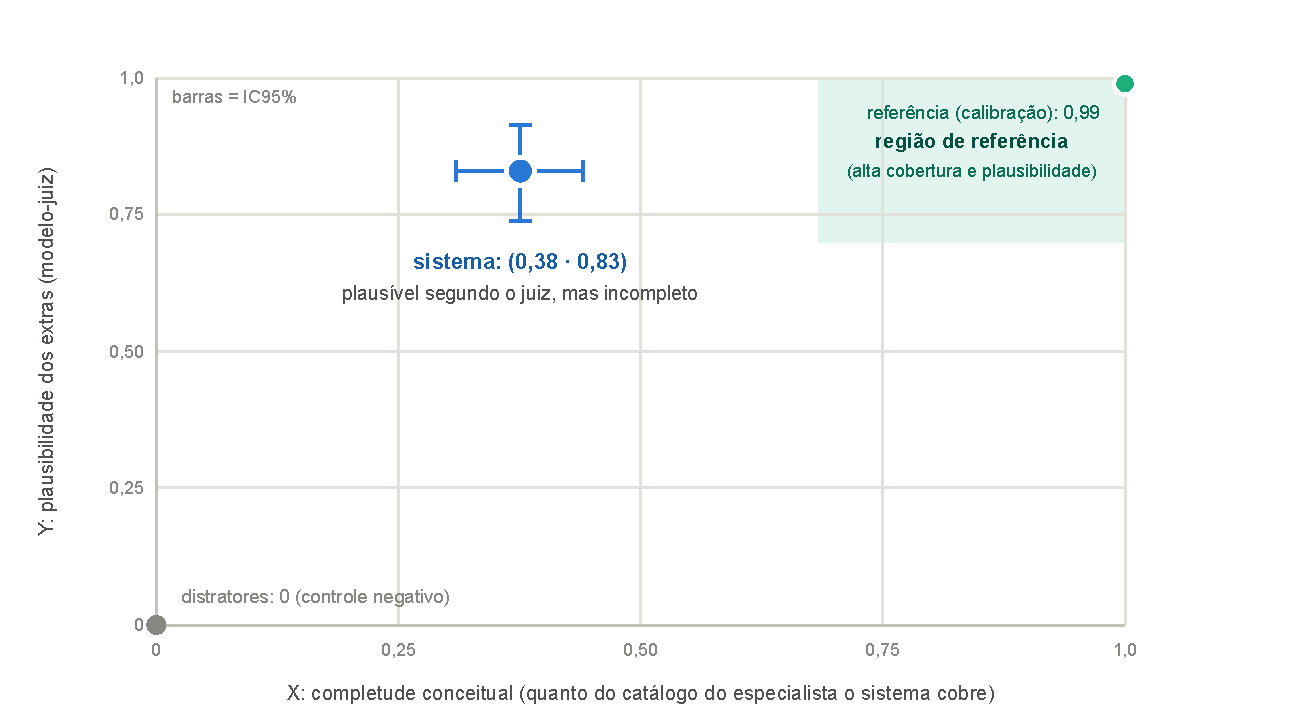
\includegraphics[width=0.88\linewidth]{figures/figura-10.pdf}
  \caption{Síntese histórica da Campanha 1 no plano cobertura--plausibilidade. A ordenada é uma avaliação de juiz único e não uma probabilidade de validade pedagógica; a figura documenta o instrumento v1 e não representa os desfechos da Campanha 4.}
  \label{fig:c1-historica}
\end{figure}
\FloatBarrier

\subsection{Cobertura por tipo e efeito de múltiplas chamadas}

\begingroup
\small
\setlength{\tabcolsep}{4pt}
\begin{longtable}{@{}P{6.1cm}R{1.8cm}R{2.6cm}R{2.6cm}@{}}
\caption{Cobertura histórica por tipo de erro no baseline da Campanha 2.}\label{tab:error-types}\\
\toprule
Tipo na referência & N & Uma execução & União de três \\
\midrule
\endfirsthead
\toprule
Tipo na referência & N & Uma execução & União de três \\
\midrule
\endhead
Fração incorreta, por exemplo $2/4$ quando a resposta é $3/4$ & 30 & 39\% & 73\% \\
Numerador isolado, por exemplo ``3'' & 24 & 50\% & 79\% \\
Denominador isolado, por exemplo ``4'' & 24 & 14\% & 33\% \\
Outros inteiros & 5 & 73\% & 80\% \\
\textbf{Total} & \textbf{83} & \textbf{37\%} & \textbf{64\%} \\
\bottomrule
\end{longtable}
\endgroup

O ganho da união mostra diversidade entre chamadas, mas não estabelece que todos os itens adicionais sejam utilizáveis. Na Campanha 4 aparece uma segunda limitação: mesmo quando itens são gerados, o extrator pode removê-los antes do grafo. A decisão de repetir chamadas precisa, portanto, considerar quatro custos simultaneamente: API, revisão pedagógica, complexidade estrutural e taxa efetiva de retenção.

\subsection{Testes pareados selecionados da Campanha 2}

As diferenças foram calculadas dentro do exercício e avaliadas por permutação exata com ajuste de Holm. A tabela preserva os resultados que orientaram a interpretação; ela não transforma ausência de significância em equivalência.

\begingroup
\small
\setlength{\tabcolsep}{3pt}
\begin{longtable}{@{}P{5.3cm}C{3.0cm}C{1.8cm}C{1.8cm}P{2.2cm}@{}}
\caption{Comparações históricas contra o Gemini na Campanha 2.}\label{tab:c2-tests}\\
\toprule
Comparação & $\Delta$ médio [IC95\%] & p exato & p-Holm & Resultado \\
\midrule
\endfirsthead
\toprule
Comparação & $\Delta$ médio [IC95\%] & p exato & p-Holm & Resultado \\
\midrule
\endhead
GLM-5.2, completude conceitual & $+0,047$ [$-0,048$; 0,143] & 0,381 & 0,988 & não detectado \\
DeepSeek, completude conceitual & $+0,003$ [$-0,089$; 0,091] & 0,957 & 0,988 & não detectado \\
Claude Sonnet 5, completude conceitual & $+0,047$ [$-0,038$; 0,142] & 0,329 & 0,988 & não detectado \\
DeepSeek, completude de passos & $-0,031$ [$-0,047$; $-0,015$] & 0,003 & 0,035 & diferença detectada \\
DeepSeek, F1 estrutural & $-0,056$ [$-0,092$; $-0,023$] & 0,005 & 0,052 & limítrofe após Holm \\
Claude Sonnet 5, inclusão de traços & $+0,059$ [0,017; 0,101] & 0,011 & 0,114 & não após Holm \\
\bottomrule
\end{longtable}
\endgroup

\section{Método e resultados completos da Campanha 3}

\subsection{Bateria e estimandos}

O protocolo v2 gerou a entrada sem abrir o conteúdo comportamental do BRD. A bateria, por outro lado, não era integralmente independente da referência: 375 de 636 itens derivavam dela, e 261 eram sondas construídas do gabarito.

\begin{table}[htbp]
\centering
\caption{Composição da bateria comportamental da Campanha 3.}
\label{tab:c3-battery}
\small
\begin{tabularx}{\textwidth}{@{}P{3.4cm}Y R{1.8cm}@{}}
\toprule
Família & Origem e função & Itens \\
\midrule
A --- referência & 24 traços corretos, 192 ações buggy e 24 pedidos de dica & 240 \\
B --- mutações & traços perturbados derivados da referência & 135 \\
C --- sondas & itens de domínio oriundos do gabarito; verdadeiros negativos & 261 \\
\midrule
Total & 24 a 28 itens por exercício & 636 \\
\bottomrule
\end{tabularx}
\end{table}

Para cada ação buggy, \Rbug{} verifica se o executor aceita a ação como erro previsto no estado correspondente. Para cada caminho correto, \Rok{} exige aceitação integral e chegada ao objetivo. A sensibilidade \Rbuganchor{} remove 42 ações mecânicas que não puderam ser ancoradas; \Rokcompleted{} relaxa a igualdade de caminho e exige apenas conclusão. A cobertura por valor ignora estado e ordem e, por isso, é secundária.

\subsection{Nove condições}

\begingroup
\footnotesize
\setlength{\tabcolsep}{3pt}
\begin{longtable}{@{}P{4.2cm}C{2.5cm}C{1.4cm}C{2.6cm}C{2.5cm}@{}}
\caption{Desfechos e cobertura nas nove condições da Campanha 3.}\label{tab:c3-all-arms}\\
\toprule
Condição & \Rbug{} [IC95\%] & \Rok{} & Cobertura [IC95\%] & Sinal mole \\
\midrule
\endfirsthead
\toprule
Condição & \Rbug{} [IC95\%] & \Rok{} & Cobertura [IC95\%] & Sinal mole \\
\midrule
\endhead
Baseline Gemini & 0,054 [0,016; 0,095] & 0 & 0,243 [0,163; 0,324] & 0/72 \\
GLM-5.2 & 0,040 [0,016; 0,068] & 0 & 0,178 [0,122; 0,236] & 0/72 \\
DeepSeek V4 Pro & 0,023 [0,010; 0,036] & 0 & 0,199 [0,143; 0,260] & 0/72 \\
Catálogo interno & 0,021 [0,005; 0,040] & 0 & 0,215 [0,152; 0,282] & 0/72 \\
Limite de seis candidatos & 0,078 [0,028; 0,134] & 0 & 0,419 [0,342; 0,495] & 61/72 \\
Saturação textual & 0,042 [0,010; 0,082] & 0 & 0,238 [0,171; 0,307] & 0/72 \\
DOM inválido para inferência & 0,028 [0,005; 0,056] & 0 & 0,207 [0,134; 0,279] & 0/72 \\
Screenshot inválido para inferência & 0,023 [0,009; 0,036] & 0 & 0,251 [0,180; 0,324] & 0/72 \\
Chamada única & 0,010 [0; 0,024] & 0 & 0,203 [0,147; 0,264] & 1/72 \\
\bottomrule
\end{longtable}
\endgroup

Os braços DOM e screenshot permanecem na tabela para preservar a trilha, mas não recebem interpretação causal. O resultado do limite de seis candidatos demonstra aumento de cobertura por valor; não demonstra melhora comportamental e coincide com maior frequência de alerta estrutural.

\subsection{Sensibilidades da Campanha 3}

\begingroup
\footnotesize
\setlength{\tabcolsep}{3pt}
\begin{longtable}{@{}P{5.0cm}C{3.7cm}C{3.7cm}@{}}
\caption{Sensibilidades exploratórias da Campanha 3.}\label{tab:c3-sens}\\
\toprule
Condição & \Rbuganchor{} [IC95\%] & \Rokcompleted{} [IC95\%] \\
\midrule
\endfirsthead
\toprule
Condição & \Rbuganchor{} [IC95\%] & \Rokcompleted{} [IC95\%] \\
\midrule
\endhead
Baseline & 0,065 [0,020; 0,113] & 0,069 [0; 0,167] \\
GLM-5.2 & 0,048 [0,019; 0,080] & 0,042 [0; 0,111] \\
DeepSeek & 0,027 [0,013; 0,044] & 0,097 [0,042; 0,167] \\
Catálogo interno & 0,025 [0,006; 0,049] & 0,097 [0; 0,222] \\
Limite de seis candidatos & 0,094 [0,037; 0,157] & 0,125 [0,042; 0,236] \\
Saturação & 0,050 [0,014; 0,096] & 0,083 [0; 0,194] \\
DOM, não interpretável & 0,033 [0,007; 0,066] & 0,292 [0,125; 0,472] \\
Screenshot, não interpretável & 0,030 [0,012; 0,049] & 0,014 [0; 0,042] \\
Chamada única & 0,014 [0; 0,032] & 0 [0; 0] \\
\bottomrule
\end{longtable}
\endgroup

Os relatórios históricos não retiveram o veredito de cada ação. O numerador de \Rbug{} foi reconstruído a partir da taxa ancorável e do denominador conhecido, com tolerância de arredondamento e teste de regressão. Outros matchers não podem ser recomputados item a item sem nova execução. Essa limitação é uma razão adicional para manter a Campanha 3 como evidência histórica secundária.

\section{Análises invalidadas e incidentes preservados}

\begin{enumerate}
  \item \textbf{Envelope v1 derivado do BRD.} A entrada das Campanhas 1--2 e a referência vinham do mesmo arquivo. Testes impediam campos proibidos, mas não demonstravam independência semântica.
  \item \textbf{Braço DOM.} A representação compartilhada continha um enunciado veterinário alheio aos exercícios. Seus contrastes não medem efeito de DOM válido.
  \item \textbf{Braço screenshot.} A imagem do exercício \path{00bubble} foi usada nos 24 exercícios. Seus resultados não medem efeito visual corretamente pareado.
  \item \textbf{Painel da Campanha 3.} O coletor esperava \path{extras}, enquanto os relatórios gravavam \path{extra}. Os 179 itens julgados incluíam 83 itens da referência e 96 controles, mas zero excedente do sistema. Os kappas não apoiam alegações sobre saídas dos agentes.
  \item \textbf{Denominador de \Rbug{}.} A implementação inicial excluiu 42 ações mecânicas; a análise corrigida restaura as 192 ações planejadas e mantém 150 ancoráveis como sensibilidade.
  \item \textbf{Painéis técnicos da Campanha 4.} Lançamentos v1, v2 e v4 foram excluídos integralmente por incompatibilidades de schema, gramática e mudança de composição. Nenhum escore foi reaproveitado no painel final.
  \item \textbf{Concordância degenerada.} Dez dimensões constantes do painel final eram exibidas como alfa/kappa 1. A errata v5.1 as marca como não estimáveis; as notas brutas permanecem inalteradas.
\end{enumerate}

Registrar esses incidentes não enfraquece a rastreabilidade; impede que correções técnicas sejam confundidas com seleção favorável de resultados. Nenhum resultado invalidado é usado na conclusão consolidada.

\section{Engenharia e limites do GraphForge}

\begin{figure}[tbp]
  \centering
  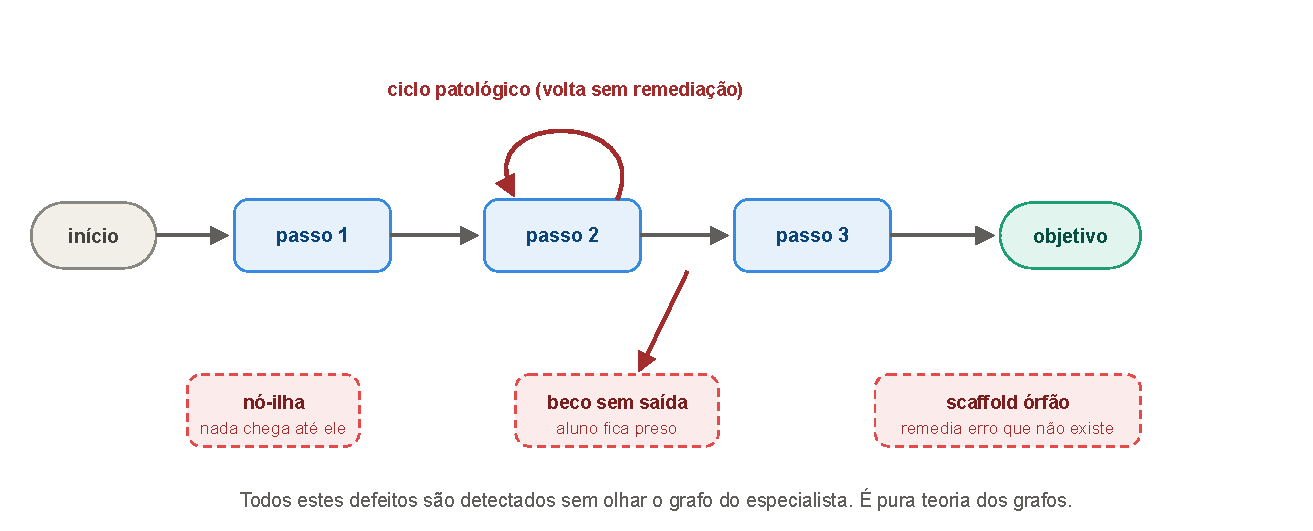
\includegraphics[width=0.92\linewidth]{figures/figura-08.pdf}
  \caption{Exemplos conceituais de violações estruturais procuradas pelo verificador. A ausência desses defeitos não implica conteúdo pedagogicamente correto.}
  \label{fig:structural-defects}
\end{figure}
\FloatBarrier

\begingroup
\small
\setlength{\tabcolsep}{3pt}
\begin{longtable}{@{}P{3.4cm}P{6.0cm}P{4.6cm}@{}}
\caption{Camadas de evidência estrutural do GraphForge.}\label{tab:graphforge-evidence}\\
\toprule
Ensaio & Resultado & Alegação permitida \\
\midrule
\endfirsthead
\toprule
Ensaio & Resultado & Alegação permitida \\
\midrule
\endhead
Testes de propriedades & 10.000 configurações aleatórias sem violação dura implementada & robustez observada dentro da taxonomia e do gerador de casos \\
Mutation testing & 260/260 mutantes detectados em dez classes; bases intactas sem sinal espúrio & sensibilidade e especificidade para as mutações cobertas \\
Campanha 3 & 0/648 violações duras; 62/648 sinais moles & conformidade estrutural dura nos grafos observados; alertas de complexidade persistem \\
Campanha 4 & 34/34 pares de reexecução idênticos & determinismo observado para configurações operacional e de capacidade \\
Transporte C4 & perdas antes e depois da configuração & montador não pode recuperar campos que não recebe \\
\bottomrule
\end{longtable}
\endgroup

Determinismo, integridade estrutural e validade pedagógica são propriedades diferentes. O GraphForge pode reproduzir exatamente uma topologia que contém conteúdo incompleto; também pode satisfazer todas as invariantes e ainda organizar uma remediação inadequada. O verificador deve permanecer como gate de engenharia, acompanhado de gates separados de schema, conteúdo, transporte e revisão pedagógica.

\section{Registro de modelos, funções e custos}

\begingroup
\footnotesize
\setlength{\tabcolsep}{3pt}
\begin{longtable}{@{}P{1.25cm}P{3.0cm}P{4.1cm}P{3.7cm}P{2.2cm}@{}}
\caption{Modelos e custos por campanha; valores históricos aproximados não devem ser somados como cobrança exata.}\label{tab:model-cost-registry}\\
\toprule
Fase & Objeto & Gerador(es) & Juiz(es) & Custo declarado \\
\midrule
\endfirsthead
\toprule
Fase & Objeto & Gerador(es) & Juiz(es) & Custo declarado \\
\midrule
\endhead
C1 & bancada integrada & Gemini 3.5 Flash & GLM-4.5 & aprox. US\$ 4 \\
C2 & robustez histórica & Gemini 3.5 Flash; GLM-5.2; DeepSeek V4 Pro; Claude Sonnet 5 & Mistral Large comum aos braços & aprox. US\$ 30 \\
C3 & conformidade e ablações & Gemini; braços GLM e DeepSeek; ablações & painel planejado sem validade sobre excedentes & US\$ 16,72 em 1.970 chamadas \\
C4 geração & agentes implantados & Gemini 3.5 Flash & não aplicável & US\$ 1,9540 \\
C4 painel final & saídas congeladas & não aplicável & GLM-5.2; Qwen 3.7 Plus; DeepSeek V4 Pro & US\$ 1,2432 conservador \\
C4 lançamentos excluídos & testes técnicos & não aplicável & composições técnicas anteriores & US\$ 2,2211 conhecido, incompleto \\
\bottomrule
\end{longtable}
\endgroup

Os custos aproximados das Campanhas 1 e 2 provêm da narrativa operacional e não possuem journal de chamadas suficiente para reconciliação financeira independente; são mantidos somente como ordem de grandeza. O custo da Campanha 3 reconcilia 1.970 registros e inclui dois erros primários seguidos de fallback bem-sucedido, portanto houve zero falha \emph{final} de autoria, não zero falha de chamada. Os modelos históricos Claude e GPT não pertencem ao painel final da Campanha 4. Claude aparece apenas como gerador de um braço da Campanha 2 e em lançamento técnico excluído; GPT aparece somente em planejamento e lançamento excluído. A mudança do painel não altera as saídas Gemini, as métricas determinísticas ou o GraphForge; altera apenas a evidência subjetiva auxiliar, razão pela qual o painel final é declarado pós-registro.

\section{Desvios, emendas e decisões pós-registro}

O congelamento foi local e baseado em hashes; não corresponde a registro público independente com carimbo de tempo. As emendas são preservadas para que um leitor possa distinguir decisões prospectivas de correções pós-resultado.

\begingroup
\small
\setlength{\tabcolsep}{3pt}
\begin{longtable}{@{}P{1.9cm}P{2.8cm}P{5.3cm}P{3.6cm}@{}}
\caption{Trilha resumida de emendas da Campanha 4.}\label{tab:amendments}\\
\toprule
Momento & Emenda & Motivo & Efeito analítico \\
\midrule
\endfirsthead
\toprule
Momento & Emenda & Motivo & Efeito analítico \\
\midrule
\endhead
Pré-geração & métricas v2 & contrato multi-problema, placeholders e ausência de estado/SAI & estimandos por \path{problemId}; 3b por valor; 3c estrito; transporte por campo \\
Pós-falha & retomada limitada & JSON 3b malformado no grupo 5 & estado falho não repetido; grupo 6 independente autorizado \\
Pós-resultado & errata v2.1 & vetor incorreto em quatro taxas de campo do 3a & apenas taxas descritivas corrigidas; estimandos e contagens inalterados \\
Pós-auditoria & sensibilidade por batch & quatro exercícios compartilham cada chamada & ICs descritivos por seis clusters; não substituem análise registrada \\
Pós-auditoria & cobertura do quarto KC & gate inicial enumerava três de quatro KCs; verificação operacional não reteve respostas HTTP brutas & atestação v2 qualificada como não externamente reproduzível; enriquecimento efetivo vazio e estimandos inalterados \\
Pré-painel final & schemas v2/v3 & incompatibilidade de keywords e gramáticas por unidade & lançamentos parciais excluídos; três schemas estáveis por papel \\
Pré-painel final & modelos v4/v5 & retirada de Claude e GPT por custo & painel final reiniciado com GLM, Qwen e DeepSeek; composição pós-registro declarada \\
Pós-auditoria & errata de concordância v5.1 & categoria única era exibida como alfa/kappa 1 & coeficientes degenerados marcados como não estimáveis; escores inalterados \\
\bottomrule
\end{longtable}
\endgroup

\section{Checklist para submissão editorial}

Antes da submissão a uma revista, quatro itens dependem de informação externa ao experimento automatizado:

\begin{enumerate}
  \item confirmar nome institucional, afiliação, ORCID e fonte de financiamento do autor;
  \item documentar autoria, instituição, data e licença do corpus CTAT;
  \item depositar uma versão imutável do repositório em arquivo com DOI e registrar seu hash, incluindo o script de correção de $R_{\mathrm{bug}}$ e os derivados históricos da Campanha 3;
  \item adequar estilo, extensão, anonimização e declaração de uso de IA às normas da revista escolhida.
\end{enumerate}

Nenhum desses itens autoriza alterar resultados, omitir falhas ou substituir o painel final por lançamentos excluídos.

\section*{Referências}
\addcontentsline{toc}{section}{Referências}
\begingroup\raggedright\interlinepenalty=10000
\begin{hangparas}{1.5em}{1}
ALEVEN, V.; MCLAREN, B. M.; SEWALL, J.; KOEDINGER, K. R. A new paradigm for intelligent tutoring systems: example-tracing tutors. \emph{International Journal of Artificial Intelligence in Education}, v. 19, n. 2, p. 105--154, 2009.\par

ALEVEN, V.; MCLAREN, B. M.; SEWALL, J.; VAN VELSEN, M.; POPESCU, O.; DEMI, S.; RINGENBERG, M.; KOEDINGER, K. R. Example-tracing tutors: intelligent tutor development for non-programmers. \emph{International Journal of Artificial Intelligence in Education}, v. 26, n. 1, p. 224--269, 2016.\par

AMIDEI, J.; PIWEK, P.; WILLIS, A. Rethinking the agreement in human evaluation tasks. In: \emph{Proceedings of COLING 2018}. Santa Fe: Association for Computational Linguistics, 2018.\par

BROWN, J. S.; BURTON, R. R. Diagnostic models for procedural bugs in basic mathematical skills. \emph{Cognitive Science}, v. 2, n. 2, p. 155--192, 1978.\par

EFRON, B.; TIBSHIRANI, R. J. \emph{An Introduction to the Bootstrap}. New York: Chapman \& Hall, 1993.\par

HOSKING, T.; BLUNSOM, P.; BARTOLO, M. Human feedback is not gold standard. In: \emph{International Conference on Learning Representations}. 2024.\par

KRIPPENDORFF, K. \emph{Content Analysis: an introduction to its methodology}. 4. ed. Thousand Oaks: SAGE, 2018.\par

LAKENS, D. Equivalence tests: a practical primer for t tests, correlations, and meta-analyses. \emph{Social Psychological and Personality Science}, v. 8, n. 4, p. 355--362, 2017.\par

LAKENS, D.; SCHEEL, A. M.; ISAGER, P. M. Equivalence testing for psychological research: a tutorial. \emph{Advances in Methods and Practices in Psychological Science}, v. 1, n. 2, p. 259--269, 2018.\par

PANICKSSERY, A.; BOWMAN, S. R.; FENG, S. LLM evaluators recognize and favor their own generations. In: \emph{Advances in Neural Information Processing Systems}, v. 37, 2024. DOI: 10.52202/079017-2197.\par

SHAVELSON, R. J.; WEBB, N. M. \emph{Generalizability Theory: a primer}. Newbury Park: SAGE, 1991.\par

TVERSKY, A. Features of similarity. \emph{Psychological Review}, v. 84, n. 4, p. 327--352, 1977.\par

VANLEHN, K. \emph{Mind Bugs: the origins of procedural misconceptions}. Cambridge: MIT Press, 1990.\par
\end{hangparas}
\endgroup

\end{document}
